\documentclass[a4paper,french,12pt]{article}

\usepackage[T1]{fontenc}
\usepackage[utf8]{inputenc}
\usepackage{lmodern}
\usepackage{fancyhdr}
\usepackage{nameref}
\usepackage{lastpage}
\usepackage[margin=2cm,top=1cm,bottom=1.5cm,headheight=5mm,headsep=2mm]{geometry}
\usepackage{minted}
\usepackage{setspace}
\usepackage{amsmath,amssymb,stmaryrd}
\usepackage{multirow}
\usepackage[bottom]{footmisc}
\usepackage{graphicx}
\usepackage{babel}
\usepackage{listings}
\usepackage{caption,subcaption}
\usepackage{xcolor}
\usepackage[unicode,pdfstartview = FitH,colorlinks,linkcolor=blue]{hyperref}

\title{Mathématiques ; Sujet de recherche}
\date{5/04/2019}
\author{}

\pagestyle{fancy}
\fancyhf{} % Supprimer le style de la page.
\renewcommand{\headrulewidth}{0.4pt}
\renewcommand{\footrulewidth}{0.1pt}

\fancyhead[C]{\emph{\leftmark}}
\fancyfoot[C]{\textbf{Page \thepage/\pageref{LastPage}}}

\begin{document}

\newcounter{def}
\newcommand{\newDef}[1]{\stepcounter{def} \textbf{\underline{Définition n$^{\underline{o}} \thedef$ :}} \emph{#1}}
\newcounter{prop}
\newcommand{\newprop}[1]{\stepcounter{prop} \textbf{\underline{Propriété n$^{\underline{o}} \theprop$ :}} \emph{#1}}
\newcounter{coro}
\newcommand{\newcoro}[1]{\stepcounter{coro} \textbf{\underline{Corollaire n$^{\underline{o}} \thecoro$ :}} \emph{#1}}
\newcounter{conj}
\newcommand{\newconj}[1]{\stepcounter{conj} \textbf{\underline{Conjecture n$^{\underline{o}} \theconj$ :}} \emph{#1}}
\newcounter{lemme}
\newcommand{\newlemme}[1]{\stepcounter{lemme} \textbf{\underline{Lemme n$^{\underline{o}} \thelemme$ :}} \emph{#1}}

\newcommand{\newPreuve}[1]{\emph{\underline{Preuve :}} #1}
\renewcommand*{\abstract}{\footnotesize\textbf{\emph{\underline{Résumé}}. ---}\scriptsize}
\renewcommand*{\contentsname}{\footnotesize\textbf{Table des matières}\scriptsize}

\renewcommand*{\labelitemi}{--}
\renewcommand*{\labelitemii}{$\bullet$}
\renewcommand*{\labelenumi}{{\textbf{\arabic{enumi})}}}%
\renewcommand*{\labelenumii}{{\alph{enumii})}}
\newcommand{\claim}{\hfill\square}

\definecolor{bg}{rgb}{0.95,0.95,0.95} % Couleur de fond d'écran des scriptes Python.

%---------------------------------------------------------------------------
%---------------- Première page --------------------------------------------
%---------------------------------------------------------------------------
\thispagestyle{empty}
\begin{center}
\rule[0.5ex]{\textwidth}{0.5mm}
\vspace*{0.5cm}

{\Large \textbf{Sur une coquille d'oeuf dans une pâte feuilletée} }
\vspace*{0.25cm}

\emph{par}
\vspace*{0.25cm}

{\scriptsize Barbara FRANCISCO \& Gulliver LARSONNEUR --- $1^{\text{ère}}/\text{Terminale}$ --- Lycée Saint Paul}

{\scriptsize Alexis GAUVRIT --- $2^{\text{nde}}$ --- Lycée Charles-Augustin Coulomb}

{\scriptsize Justine VANACKERE, Noé REICH, Mohammed Sid-Ali HAFS \& Adrien FRADIN --- $1^{\text{ère}}$ --- Lycée Marguerite de Valois}

\rule[0.5ex]{1.5cm}{0.1mm}

{\scriptsize Alexandre ROBUCHON --- Professeurs encadrants (Lycée Saint Paul)}

{\scriptsize Christian MÉRON \& Grégory LIORIT --- Professeurs encadrants (Lycée Charles-Augustin Coulomb)}

{\scriptsize Cédric GOUYGOU \& Clément IZARD --- Professeurs encadrants (Lycée Marguerite de Valois)}

\rule[0.5ex]{1.5cm}{0.1mm}

{\scriptsize Charles DOSSAL --- Enseignant-Chercheur à l'INSA de Toulouse et l’Institut de Mathématiques de Toulouse}

\vspace*{0.5cm}
\emph{Les $5-6-7$ avril $2019$ à La Rochelle --- Année $2018$-$2019$}

\vspace*{0.5cm}
\rule[0.5ex]{7cm}{0.5mm}
\vspace*{0.5cm}

\end{center}

%---------------------- Résumé --------------------------------------------

\begin{abstract}
Dans cet article nous présentons nos recherches sur l'un des sujets du chercheur Charles DOSSAL. 

Nous disposons d'une pâte carrée d'un mètre de côté. Nous pouvons étaler la pâte, c'est-à-dire obtenir un rectangle de côté $2$ par $1$. Puis il faut plier la pâte pour obtenir de nouveau une pâte de $1$ mètre de côté. L'action étaler-plier constitue une \textbf{étape}, renouvelable autant de fois que nécessaire.

Mais si une coquille d'œuf se dépose dans la pâte, où se trouvera-t-elle après $3$ étapes, $4$ étapes, $n$ étapes ?
\end{abstract}

\vspace*{0.5cm}

%---------------------- Sommaire ------------------------------------------

\begin{center}
{\scriptsize \tableofcontents}
\end{center}

\clearpage

%---------------------------------------------------------------------------
%---------------- Visuel et informatique -----------------------------------
%---------------------------------------------------------------------------

\section{L'approche visuelle et informatique}
Dans cette section, nous étudions le problème sous un angle graphique et informatique. Notez toutefois que certains schémas et programmes informatique sont placés dans les autres sections pour donner à cet article une vision chronologique et non thématique.

%---------------- Présentation problème ------------------------------------

\subsection{Introduction au problème}
Le problème de la pâte feuilletée décrit en résumé consiste à prendre une pâte carrée (disons de $1$ mètre de côté) :

\vspace*{-0.5cm}

\begin{center}
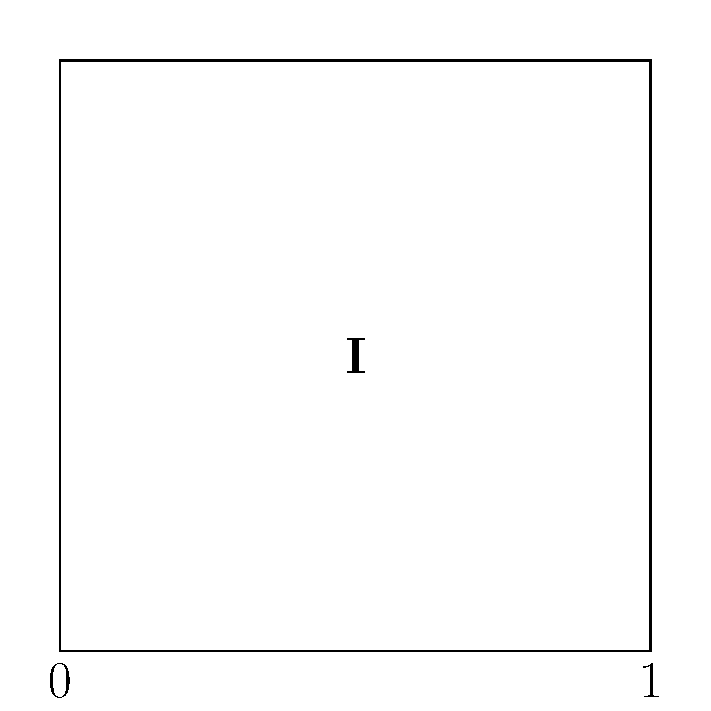
\includegraphics[scale=0.275]{../TeXGraph/Pdf/intro_pate_1.pdf}
\captionof{figure}{\emph{Une pâte feuilletée carrée de $1$ mètre de côté}.}
\end{center}
puis, à étaler cette pâte de manière à obtenir un rectangle de $2$ mètres par $1$ mètre de côté :

\vspace*{-0.5cm}

\begin{center}
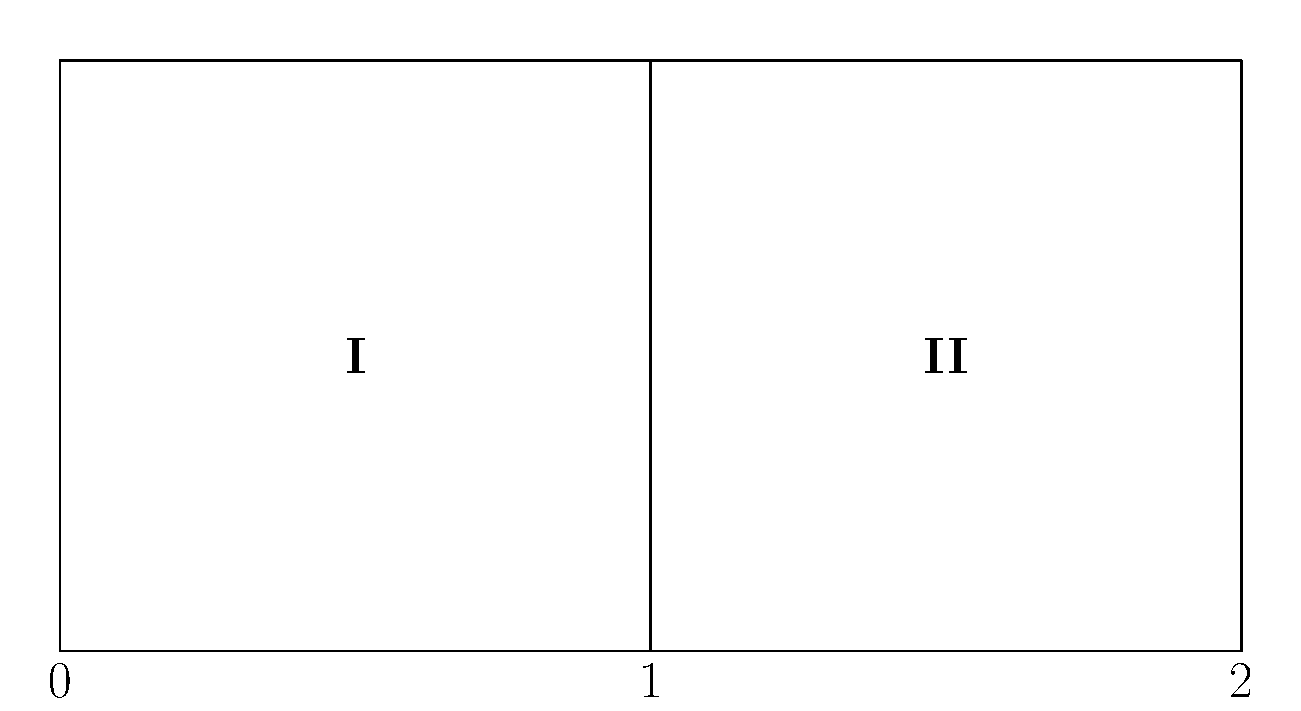
\includegraphics[scale=0.275]{../TeXGraph/Pdf/intro_pate_2.pdf}
\captionof{figure}{\emph{Une pâte feuilletée après un étalage}.}
\end{center}
et finalement, nous plions la moitié \textbf{II} du rectangle\footnote{Le pliage s'effectuera \textbf{toujours} dans le sens opposé à l'étalage.} sur l'autre de sorte à obtenir une pâte carrée (toujours de $1$ mètre de côté) :

\vspace*{-0.5cm}

\begin{center}
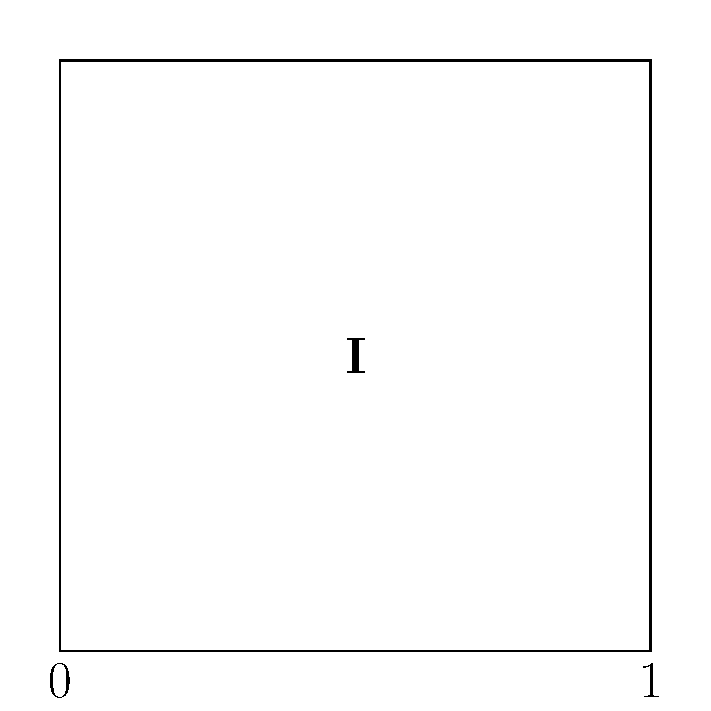
\includegraphics[scale=0.275]{../TeXGraph/Pdf/intro_pate_1.pdf}
\captionof{figure}{\emph{Une pâte feuilletée après une étape}.}
\end{center}

Mais que se passe-t-il si une coquille d'œuf (que nous modéliserons par un point) tombe dans la pâte avant une étape. Où se trouvera-t-elle après une étape, après $2$, $3$ ou $n$ étapes ? Peut-elle revenir à sa position initiale ? Peut-elle ne jamais revenir à sa position initiale ? C'est ce que nous allons voir dans la suite de cet article.

%----------------------- Schémas -----------------------------------------

\subsection{L'approche visuelle}
Dans un premier temps, nous allons étudier le problème de la pâte feuilletée au moyen d'outils visuels tels que les schémas ou les graphiques.

%----------------------- Illustration et arbre----------------------------

\subsubsection{La pâte feuilletée et la coquille d'œuf}
Visuellement\footnote{Merci à Christian MÉRON pour son animation de la pâte feuilletée. Lien vers l'animation : \emph{\href{https://scratch.mit.edu/projects/302899876/}{https://scratch.mit.edu/projects/302899876/}}.}, lorsqu'une coquille (ici un point car nous nous plaçons dans une situation \emph{idéale}) tombe dans la pâte avant une étape, deux situations (symbolisées par \textbf{A} et \textbf{B}) sont possibles :

\vspace*{-0.25cm}

\begin{center}
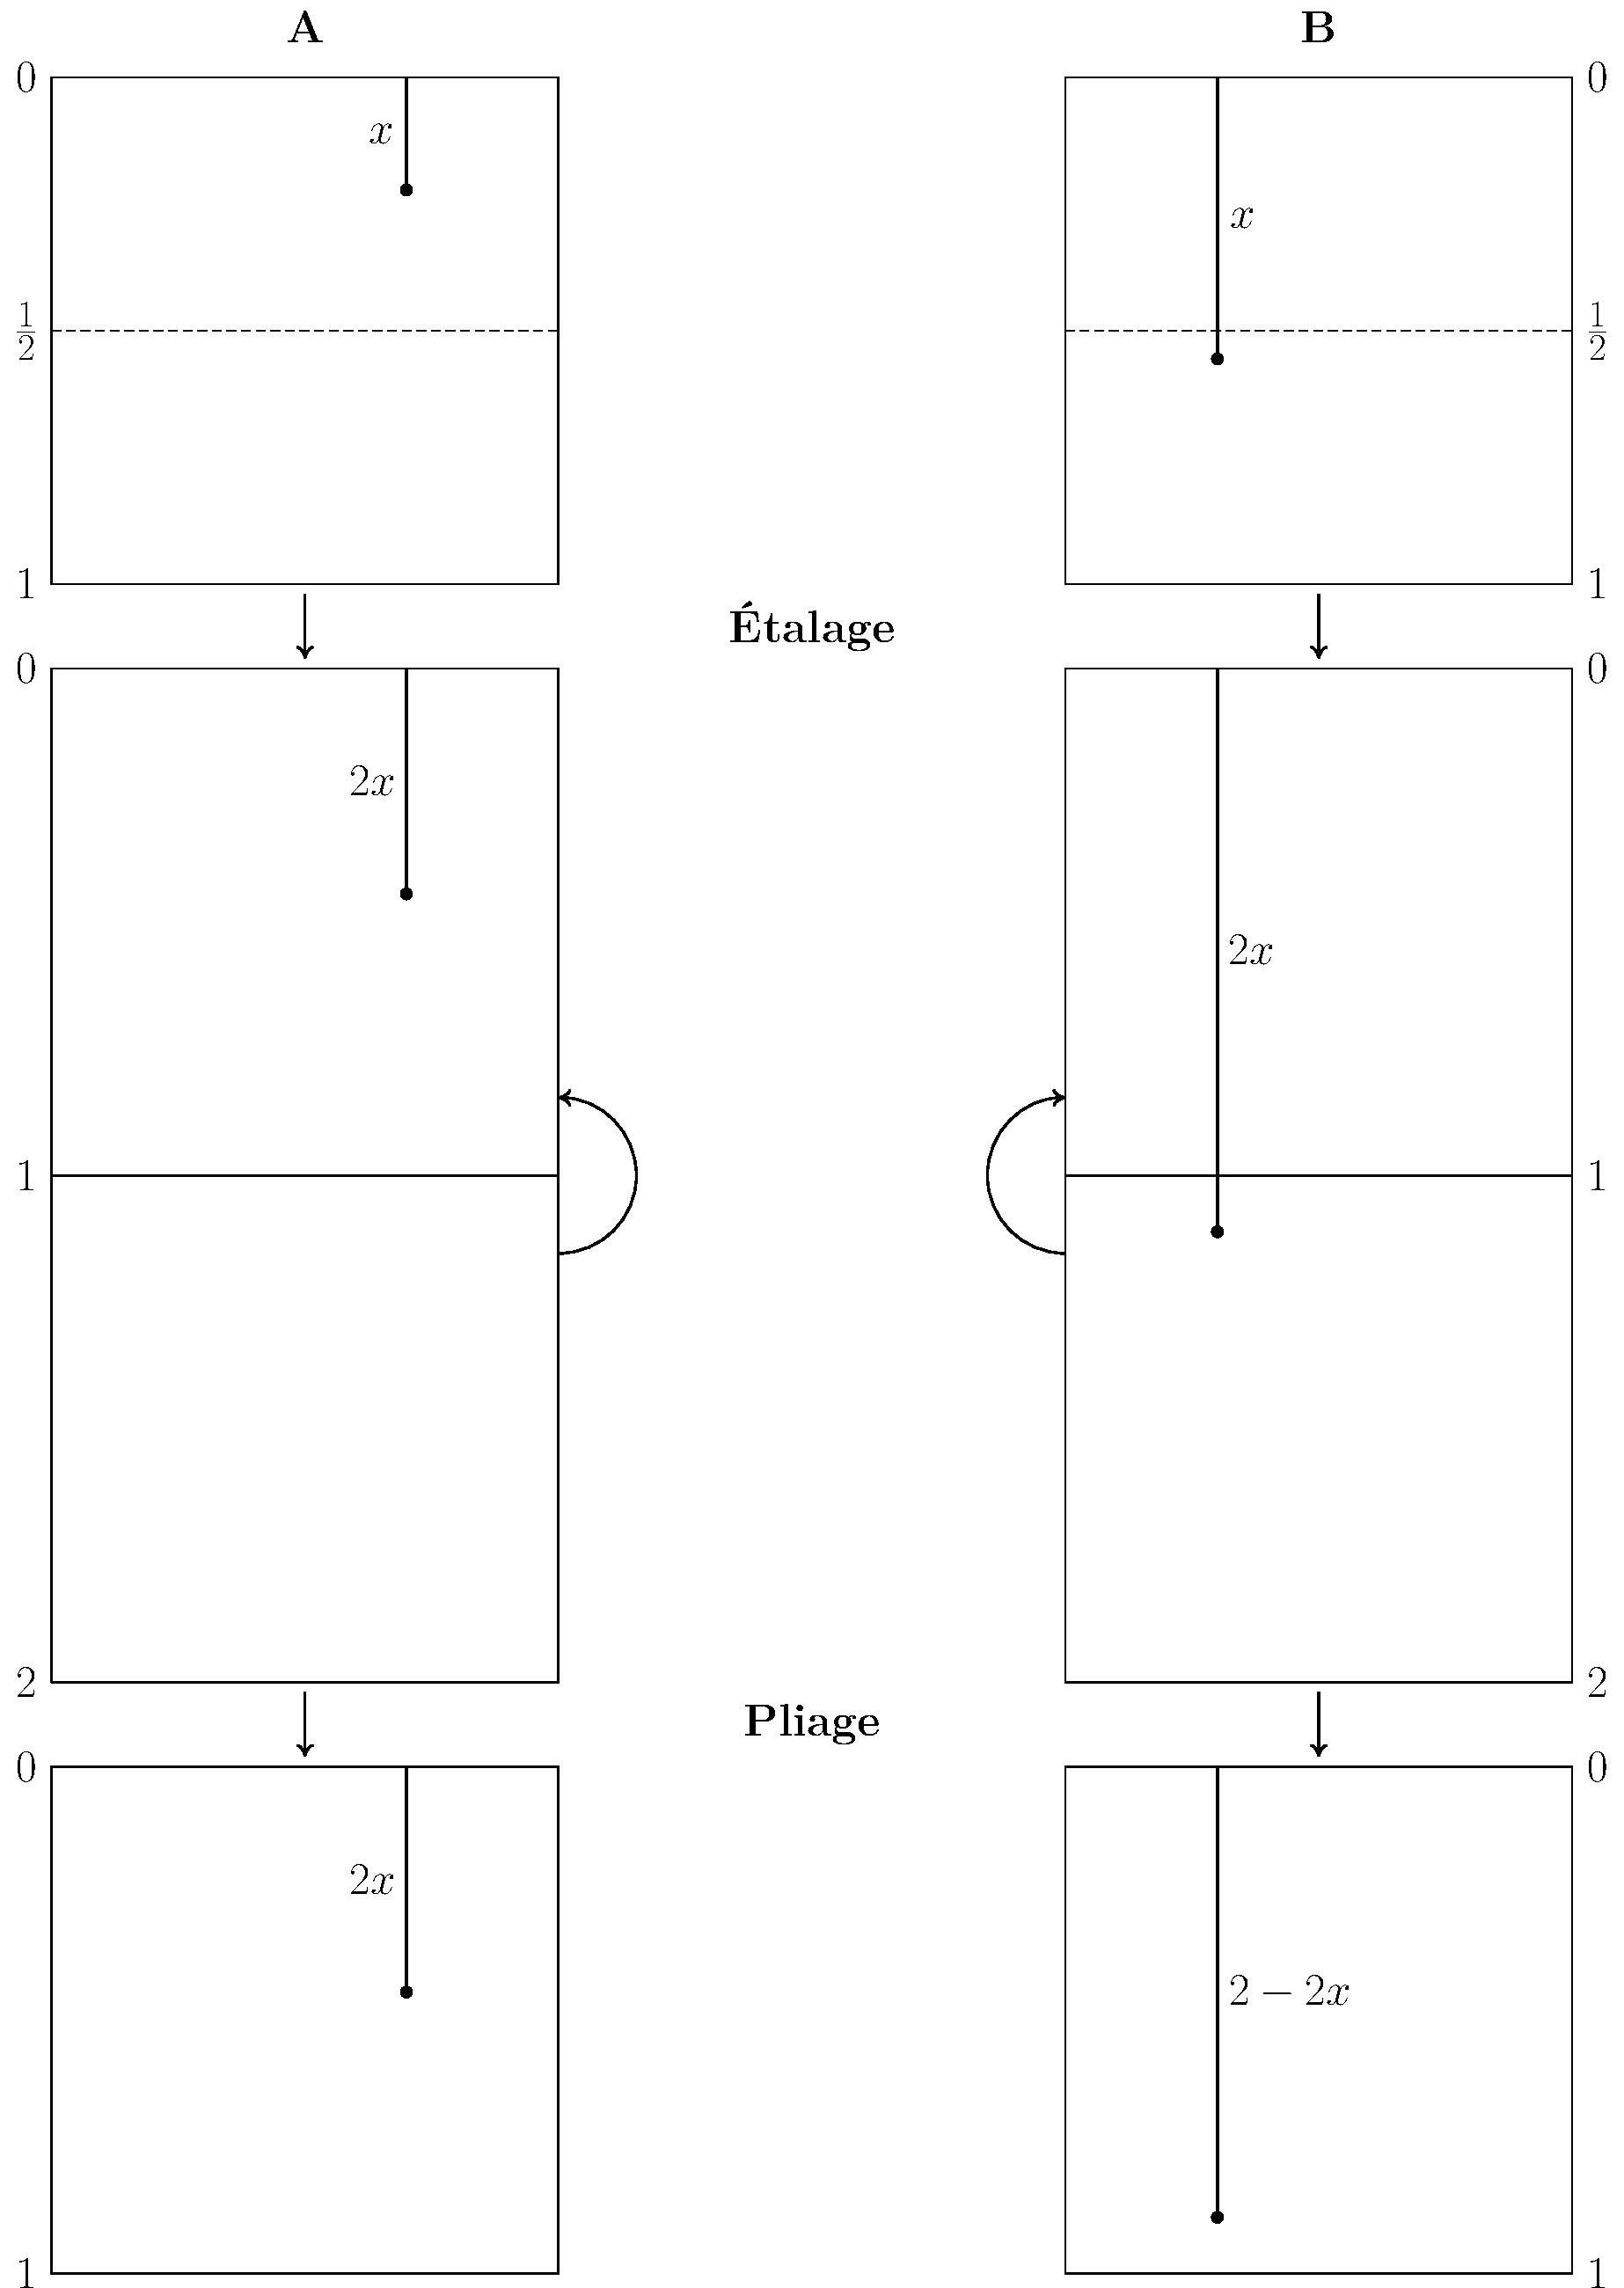
\includegraphics[scale=0.45]{../TeXGraph/Pdf/visuel_2D_pate.pdf}
\captionof{figure}{\emph{Les deux cas possibles pour une coquille après une étape}.}
\end{center}

Par convention nous noterons $x$ la position de la coquille avec $x\in\left[0;1\right]$. Dans les deux cas, après étalage, la coquille aura pour position $2x$. Dans le cas \textbf{A} puisque $x\leqslant\frac{1}{2}$ alors $2x\leqslant1$ et le pliage n'affectera pas la position de la coquille. Dans le cas \textbf{B} puisque $x>\frac{1}{2}$ alors $2x>1$ et le pliage va modifier la position de la coquille qui sera de $2-2x$ (c'est la distance qui sépare la coquille, après étalage, des deux mètres\footnote{En effet, $2x+\left(2-2x\right)=2$.} de la pâte).

Au bout d'une étape, la coquille aura comme position $2x$ ou $2-2x$. Ces modifications sont appelées les \emph{transformations du boulanger}.

Les cas \textbf{A} et \textbf{B} peuvent se résumer par un arbre :

\begin{center}
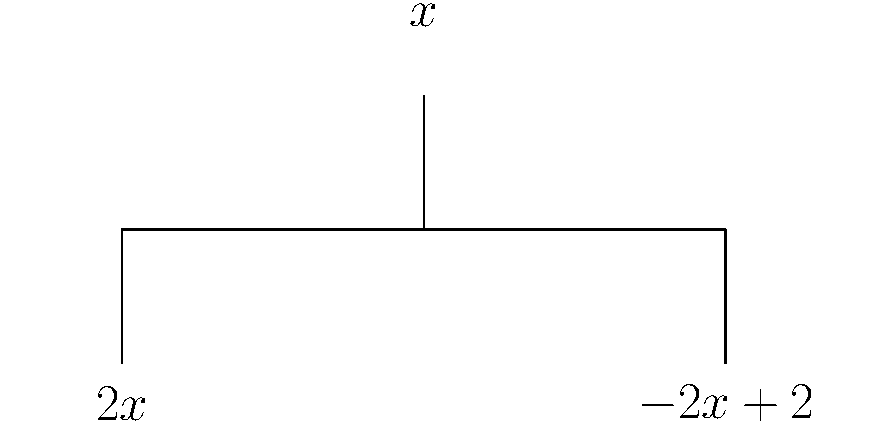
\includegraphics[scale=0.45]{../TeXGraph/Pdf/visuel_2D_arbre.pdf}
\captionof{figure}{\emph{L'arbre des positions possibles de $x$ pour une étape}.}
\end{center}
que l'on peut réitérer pour chaque nouvelles branches de l'arbre ci-dessus :

\begin{center}
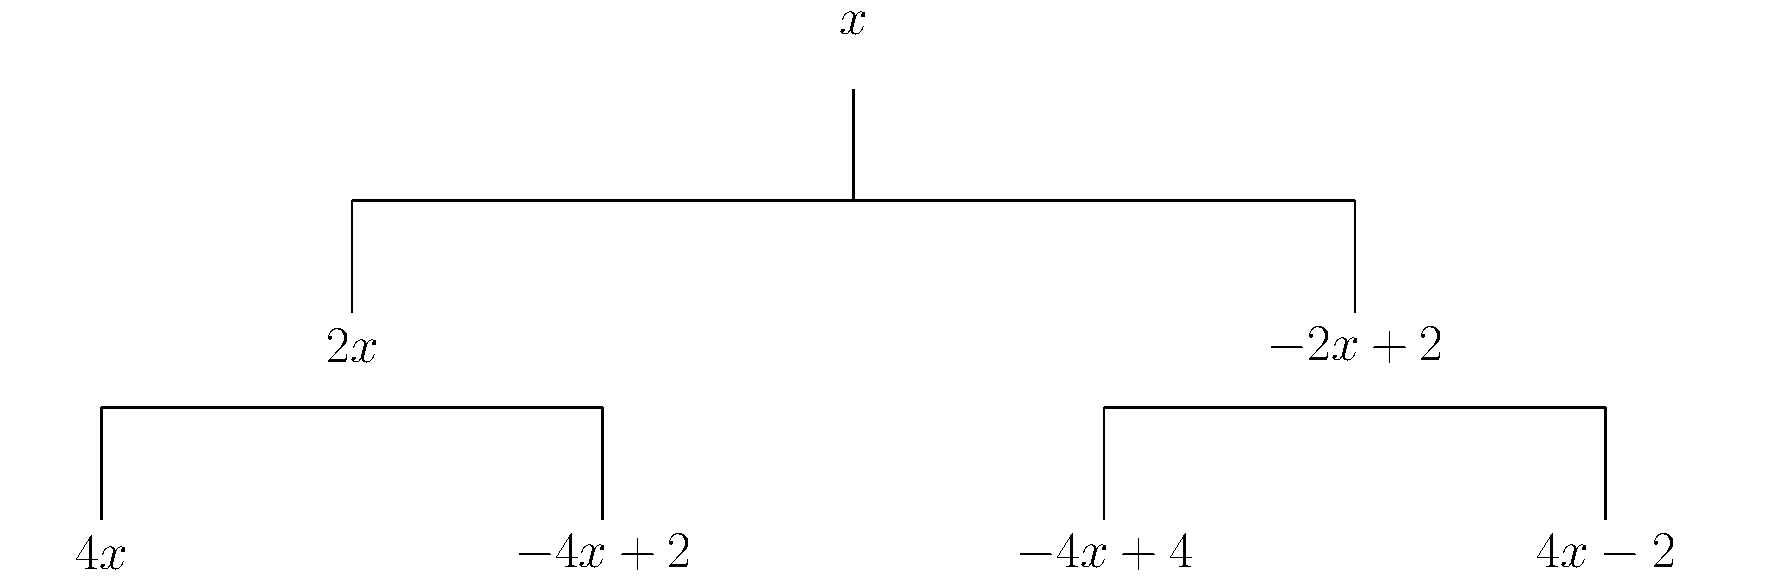
\includegraphics[scale=0.45]{../TeXGraph/Pdf/visuel_2D_arbre_2.pdf}
\captionof{figure}{\emph{L'arbre des positions possibles de $x$ pour deux étapes}.}
\end{center}
On peut alors calculer directement la position de la coquille après deux étapes selon l'intervalle auquel elle appartient : $\left[0;\frac{1}{4}\right]$, $\left]\frac{1}{4};\frac{1}{2}\right]$, $\left]\frac{1}{2};\frac{3}{4}\right]$ ou  $\left]\frac{3}{4};1\right]$. Pour chaque intervalle on utilisera une fonction particulière (respectivement) $4x$, $-4x+2$, $-4x+4$ ou $4x-2$.

%---------------- Fonction cyclique -----------------------------------

\subsubsection{La fonction et les positions périodiques}
On note $f$ la fonction qui associe à une coquille de position $x$ sa position après une étape\footnote{\hypertarget{note4}{}Notez que $f\left(x\right)=1-2\left\lvert x-\frac{1}{2}\right\rvert=1-\left\lvert2x-1\right\rvert$.} :

\vspace*{-0.4cm}

\begin{align*}
f\left(x\right)=\begin{cases}2x &\text{ si }x\leqslant\frac{1}{2}\\2-2x &\text{ si }x>\frac{1}{2}\end{cases}
\end{align*}

On peut alors représenter graphiquement $f$ :

\begin{center}
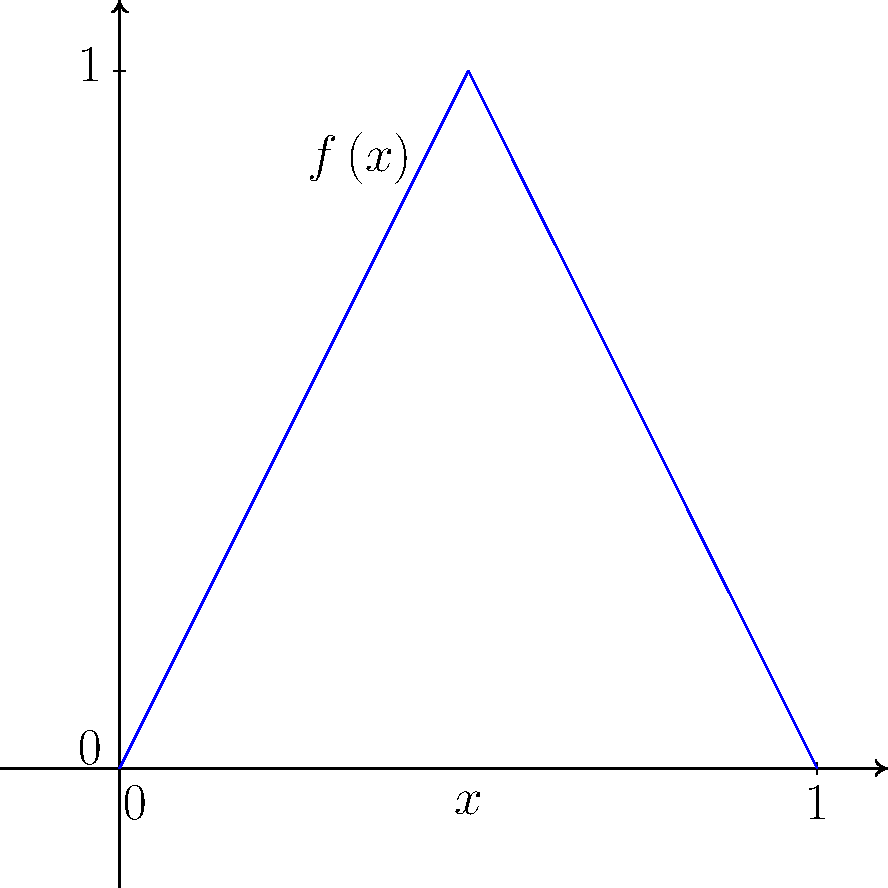
\includegraphics[scale=0.45]{../TeXGraph/Pdf/graphique_etape_1.pdf}
\captionof{figure}{\emph{Représentation graphique de $f$}.}
\end{center}
Cette représentation graphique permet de visualiser les positions périodiques c'est-à-dire, les positions où la coquille revient à sa position initiale au bout d'un certain nombre d'étape. Soit $n>0$ un entier, on note $f^n\left(x\right)=\underbrace{f(f(\ldots f}_\text{$n$ fois}(x)\ldots))$ la composée $n$-ème de $f$. Ainsi $f^n\left(x\right)$ est la position de la coquille après $n$ étapes.

\newDef{Soit un entier $n>0$, une position $x$ est $n$-périodique si $f^n\left(x\right)=x$.}

Si on cherche des positions\footnote{Nous démontrerons dans la partie mathématique qu'il y a exactement $2^n$ positions $n$-périodiques.} $1$-périodiques il suffit de tracer la droite d'équation $y=x$ et de chercher les points d'intersections :

\begin{center}
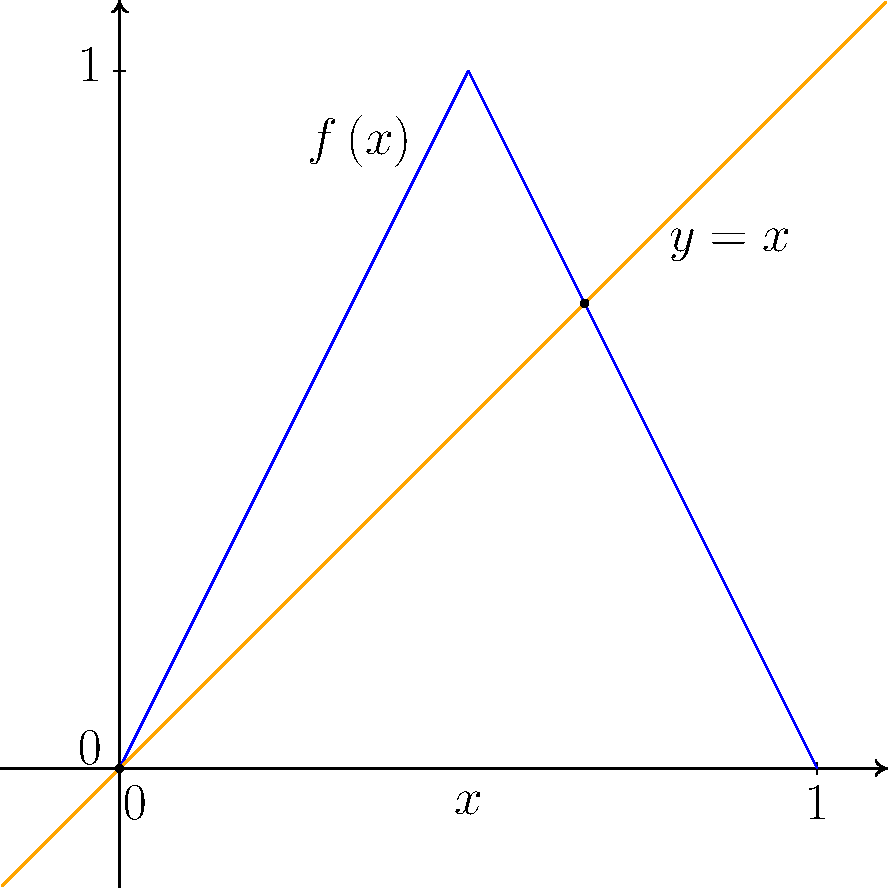
\includegraphics[scale=0.45]{../TeXGraph/Pdf/graphique_etape_1_periode.pdf}
\captionof{figure}{\emph{Les positions $1$-périodiques}.}
\end{center}

La lecture graphique montre que les points d'intersections semblent être $\left\{\left(0;0\right);\left(\frac{2}{3};\frac{2}{3}\right)\right\}$ et grâce à l'arbre de la figure $6$, si $x$ est $1$-périodique alors l'une des égalités est vraie :
\[\begin{cases}x=2x\\x=2-2x\end{cases}\]
ce qui prouve que se sont des positions $1$-périodiques. De la même façon on trouve les positions $2$-périodiques ; on trace la fonction $f^2$ et la droite $y=x$ :

\begin{center}
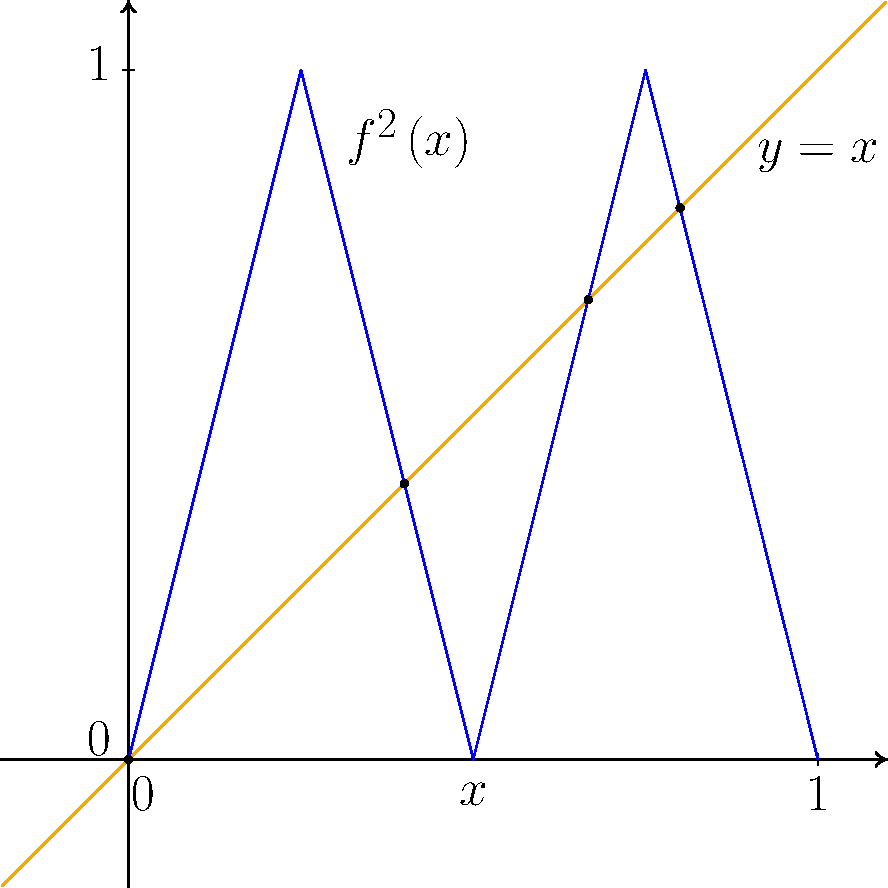
\includegraphics[scale=0.45]{../TeXGraph/Pdf/graphique_etape_2_periode.pdf}
\captionof{figure}{\emph{Les positions $2$-périodiques}.}
\end{center}
et les points d'intersections semblent être $\left\{\left(0;0\right);\left(\frac{2}{5};\frac{2}{5}\right);\left(\frac{2}{3};\frac{2}{3}\right);\left(\frac{4}{5};\frac{4}{5}\right)\right\}$ et l'arbre de la figure $6$ montre que si $x$ est $2$-périodique alors l'une des égalités est vraie\footnote{Les solutions sont $\left\{0;\frac{2}{5};\frac{2}{3};\frac{4}{5}\right\}$, c.f. \hyperlink{2}{\textbf{2 L’approche mathématiques}}.} :
\[\begin{cases}x=4x\\x=-4x+2\\x=-4x+4\\x=4x-2\end{cases}\]

%---------------- Représentation graphique --------------------------------

\subsubsection{Représentation graphique de la suite}
On considère la suite $\left(x_n\right)_{n\in\mathbb{N}}$ définie par $x_0=x$ et $x_{n+1}=f\left(x_n\right)$ que l'on souhaiterait représenter graphiquement. Pour cela on dessine la fonction $f$ et la droite $y=x$ puis, on prend un point $\left(x_0;0\right)$ et on cherche son image par $f$ :

\begin{center}
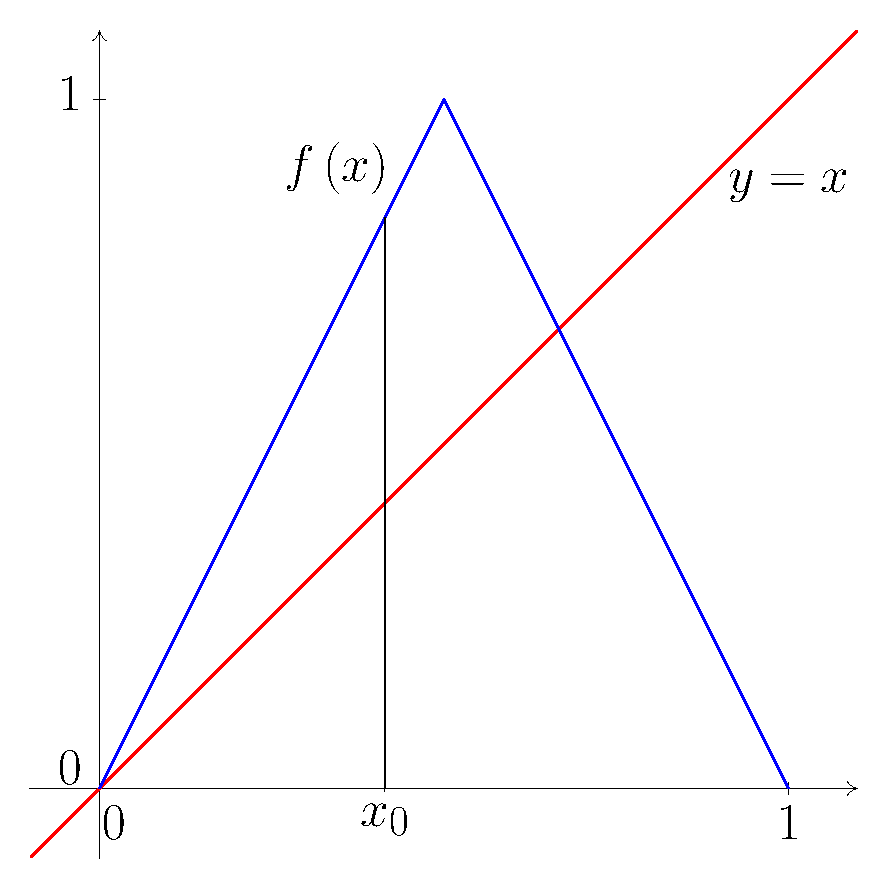
\includegraphics[scale=0.45]{../TeXGraph/Pdf/courbe_suite_image.pdf}
\captionof{figure}{\emph{Un point $\left(x_0;0\right)$ et son image par $f$}.}
\end{center}
Ensuite, on trace la droite perpendiculaire à l'axe des ordonnées passant par $\left(x_0;f\left(x_0\right)\right)$ et on cherche son intersection avec la droite $y=x$ :

\begin{center}
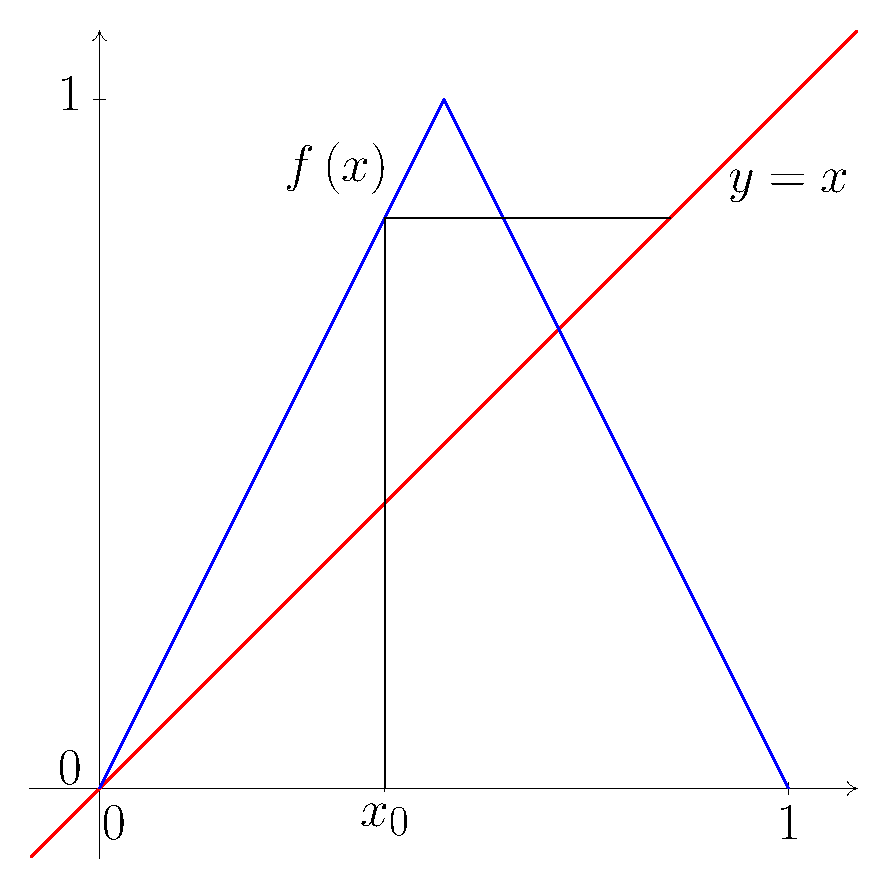
\includegraphics[scale=0.45]{../TeXGraph/Pdf/courbe_suite_intersection.pdf}
\captionof{figure}{\emph{On cherche le point $\left(f\left(x_0\right);f\left(x_0\right)\right)$}.}
\end{center}
Finalement, on projette orthogonalement le point $\left(f\left(x_0\right);f\left(x_0\right)\right)$ sur l'axe des abscisses pour obtenir le point $\left(f\left(x_0\right);0\right)$ c'est-à-dire le point $\left(x_1;0\right)$ :

\begin{center}
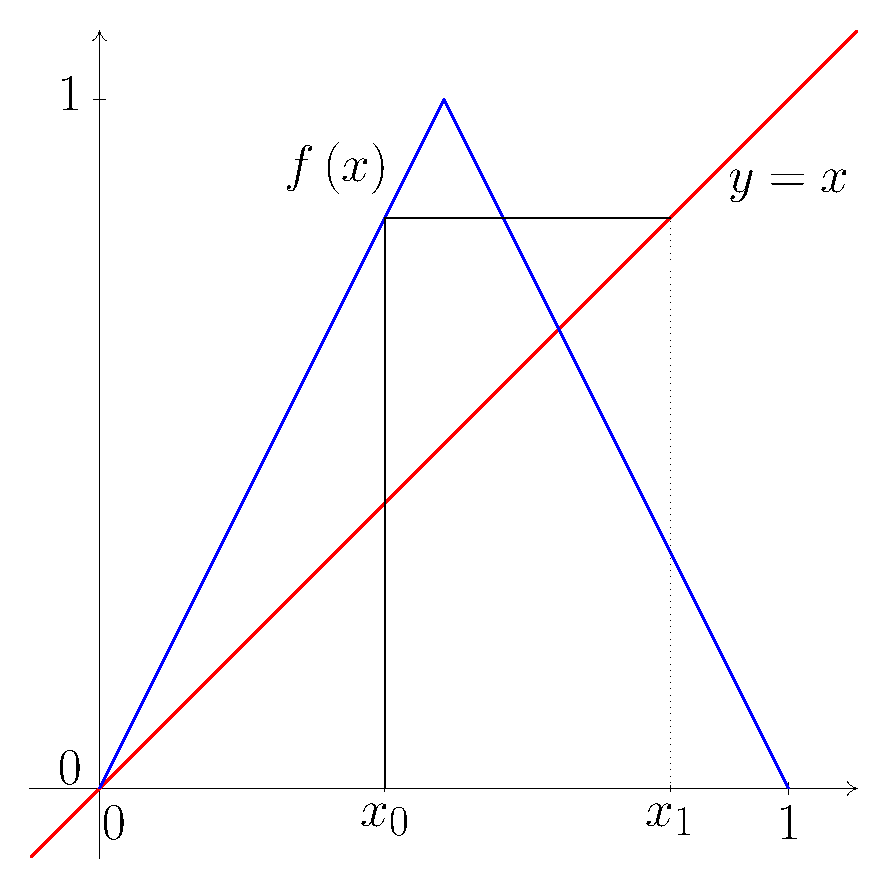
\includegraphics[scale=0.45]{../TeXGraph/Pdf/courbe_suite_x_1.pdf}
\captionof{figure}{\emph{On obtient le point $\left(x_1;0\right)$}.}
\end{center}

De la même façon\footnote{Mais à partir de $\left(x_1;0\right)$ puis de $\left(x_2;0\right)$ etc.} on construit les points $\left(x_2;0\right)$, $\left(x_3;0\right)\ldots$ En dessinant de tels graphiques pour diverses positions (des fractions comme $\frac{7}{11}$, $\frac{8}{9}$ ou des irrationnels comme $\sqrt{3}-1$, $\sqrt{10}-3$) on observe deux phénomènes :

\vspace*{-0.75cm}
\hypertarget{4}{}
\begin{center}
\begin{figure}[H]
  \begin{subfigure}[b]{0.4\textwidth}
    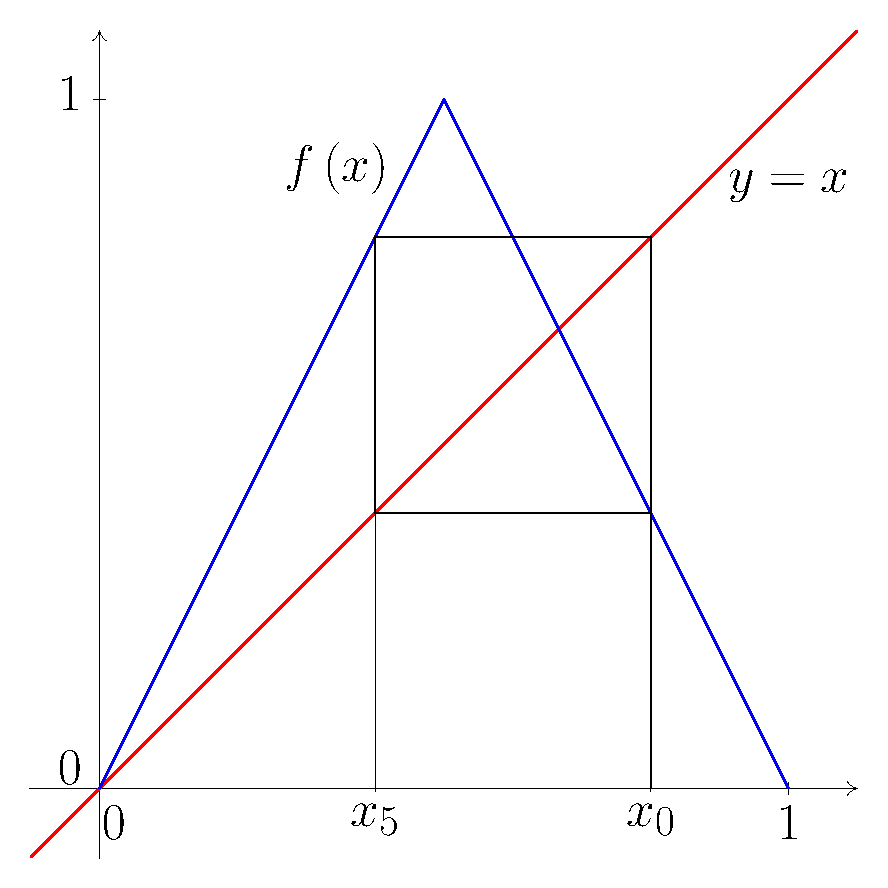
\includegraphics[scale=0.45]{../TeXGraph/Pdf/courbe_suite_phenomene_2.pdf}
    \caption{\emph{Une position périodique a un motif qui se répète}.}
    \label{fig:f1}
  \end{subfigure}
  \hfill
  \begin{subfigure}[b]{0.4\textwidth}
    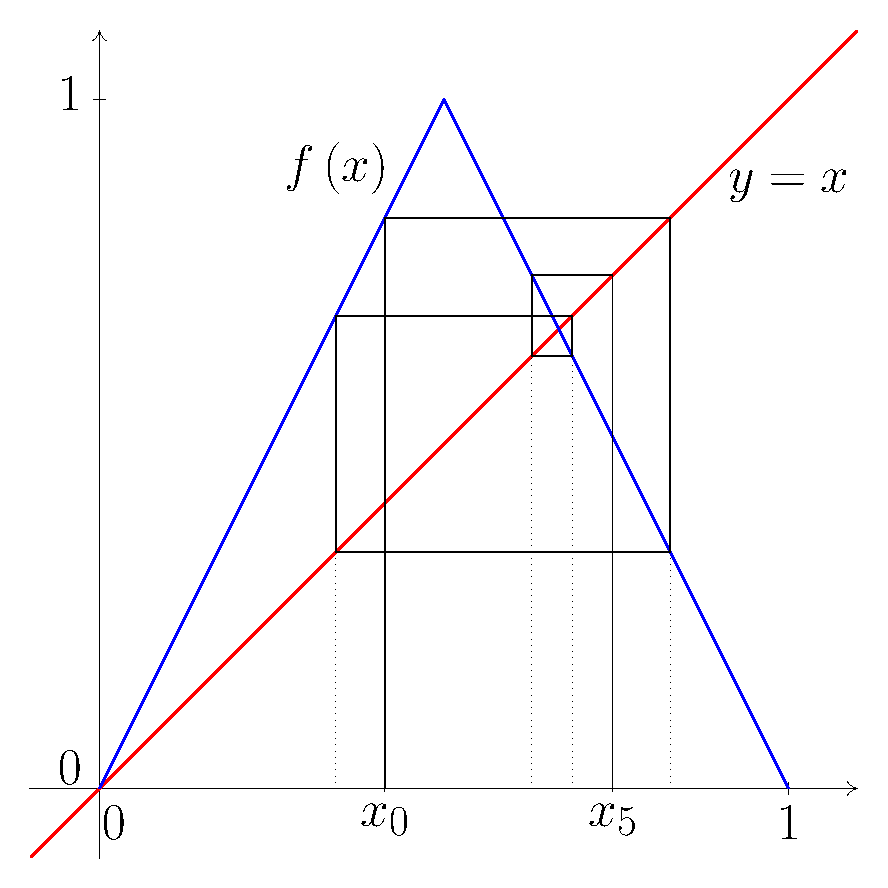
\includegraphics[scale=0.45]{../TeXGraph/Pdf/courbe_suite_phenomene_1.pdf}
    \caption{\emph{Une position (apparemment) non-périodique a motif qui ne se répète pas}.}
    \label{fig:f2}
  \end{subfigure}
  \caption{\emph{Deux phénomènes possibles, à gauche $x_0=\frac{4}{5}$ et à droite $x_0=\sqrt{2}-1$}.}
\end{figure}
\end{center}

\vspace*{-1cm}

Ces deux phénomènes correspondent à la périodicité ou non d'une position, encore faut-il prouver l'existence de positions non périodiques. Nous démontrerons plus tard l'existence de positions non périodiques (comme $\sqrt{2}-1$). 

Ainsi, l'approche visuelle permet de mieux cerner visuellement les conjectures à démontrer et offre un point de vue moins abstrait que l'approche mathématiques.

%---------------- Approche informatique -----------------------------------

\subsection{L'approche informatique}
L'approche informatique va de paire avec l'approche visuelle et permet de cadrer numériquement les conjectures à démontrer.

%---------------- Calcul des positions -----------------------------------

\subsubsection{Le calcul d'une position étape par étape}

Une première approche est de simuler par ordinateur ce qu'adviendra une position donnée après un nombre d'étapes donné. Écrivons dans un premier temps l'algorithme d'un tel programme :

\begin{center}
\begin{minted}[frame=lines,breaklines,framesep=12pt,baselinestretch=1.2,bgcolor=bg,fontsize=\footnotesize,linenos]{text}
Définir une position entre 0 et 1,
Définir un nombre d'étapes,
Tant qu'il reste des étapes :
    Si la position est entre 0 et 1/2 :
        Doubler la position,
    Sinon :
        Multiplier la position par -2 et ajouter 2,
Afficher la position.
\end{minted}
\captionof{figure}{\emph{L'algorithme qui trouve la position d'une coquille après un nombre d'étapes donné}.}
\end{center}

Les lignes $5$ et $7$ correspondent aux deux branches de l'arbre de la figure $5$ (avec $2x$ et $2-2x$). De cet algorithme on construit notre programme (en Python) :

\vspace*{-0.5cm}

\begin{center}
\begin{minted}[frame=lines,breaklines,framesep=12pt,baselinestretch=1.2,bgcolor=bg,fontsize=\footnotesize,linenos]{python}
def position_apres_etape(num,den,etape=1):
    '''Calcul de la position "num/den" après un nombre d'étapes donné.'''
    # Pour chaque étape on calcul la nouvelle position de la coquille.
    for k in range(etape):
        if 2*num>den: # Si la position est > à 1/2.
            num=2*(den-num)
        else:num*=2 # Si la position est <= 1/2 on multiplie par 2.
    # On renvoie le numérateur et le dénominateur.
    return num,den
\end{minted}
\captionof{figure}{\emph{Le code source du programme Python}.}
\end{center}

Pour les calculs aux lignes $6-7$, si $x$ est une position rationnelle\footnote{Un nombre rationnel peut s'écrire comme le quotient d'un entier relatif par un entier naturel non nul. Dans notre cas on se limitera aux entiers naturels.} alors $x=\frac{p}{q}$ avec $p,q\in\mathbb{Z}\ \left(q\not=0\right)$. On a alors les transformations du boulanger : $2x=\frac{2p}{q}$ ou $2-2x=2-\frac{2p}{q}=\frac{2\left(q-p\right)}{q}$ selon que $x\leqslant\frac{1}{2}$ ou $x>\frac{1}{2}$.

D'ailleurs, d'après la note \hyperlink{note4}{$4$} les lignes $5-6-7$ peuvent être remplacées par \mintinline{python}{num=den-abs(2*num-den)}. En effet :\hypertarget{3}{}
\[f\left(x\right)=1-\left\lvert2x-1\right\rvert=1-\left\lvert\frac{2p}{q}-1\right\rvert=1-\left\lvert\frac{2p-q}{q}\right\rvert=\frac{q-\left\lvert2p-q\right\rvert}{q}\]
car $q>0$.

Dans le cadre de notre programme, nous avons opté pour des positions rationnelles (sous la forme de fractions) car un ordinateur ne peut représenter un nombre que par une quantité finie de bits. Ainsi, toute position avec un nombre \emph{infini} de décimales\footnote{Comme $\sqrt{2}$ ou $\frac{1}{3}$. Toutefois, pour les positions rationnelles, la séparation numérateur/dénominateur corrige ce problème.} sera tronquée par un nombre fini de décimales. 

De ce fait, l'approche informatique ne nous révélera pas si une position irrationnelle est périodique ou non. Mais par contre, elle nous renseigne sur la périodicité ou non de positions rationnelles. Par exemple, $\frac{1}{3}$ n'est pas périodique car après une étape on obtiendra $\frac{2}{3}$ qui est $1$-périodique. $\frac{3}{5}$ aussi n'est pas périodique car $f\left(\frac{3}{5}\right)=2-\frac{6}{5}=\frac{4}{5}$ et $f\left(\frac{4}{5}\right)=2-\frac{8}{5}=\frac{2}{5}$ qui donne $\frac{4}{5}$ après une troisième étape.

%---------------- Calcul des périodes -----------------------------------

\subsubsection{Le calcul de la période d'une position}
Maintenant que nous pouvons calculer la position de la coquille après une étape, nous allons par un programme chercher à savoir si une position est périodique ou non. Afin de rendre les résultats rigoureux, nous ne demandons que des positions rationnelles\footnote{Comme dit dans une précédente remarque, les nombres irrationnels seront tronqués par des rationnels pour effectuer les calculs informatiques.}. Tout d'abord voici l'algorithme d'un tel programme :

\begin{center}
\begin{minted}[frame=lines,breaklines,framesep=12pt,baselinestretch=1.2,bgcolor=bg,fontsize=\footnotesize,linenos]{text}
Importer la fonction 'position_apres_etape',
Définir une position entre 0 et 1,
Définir un nombre d'étape maximal (si jamais la position n'est pas périodique),
Tant que le nombre maximal d'étape n'est pas atteint :
    Effectuer une étape,
    Modifier l'ancien numérateur par celui obtenue au-dessus,
    Si ce nouveau numérateur est égal au numérateur initial :
        Afficher que la position est périodique et sa période,
Afficher que la position ne se répète avant le nombre d'étape maximal fixé.
\end{minted}
\captionof{figure}{\emph{L'algorithme qui trouve la période d'une positions donnée (si celle-ci est périodique)}.}
\end{center}
Pour éviter de créer une \emph{boucle infinie} nous fixons un nombre d'étape maximal ($1000$ par défaut\footnote{Ce nombre d'étape maximal peut être automatiquement fixé au dénominateur de la position choisie. Pour plus d'explication, voir \hyperlink{1}{\textbf{2.4 L'étude des positions non périodiques}}.}). De cet algorithme on construit notre programme (en Python) :

\vspace*{-0.5cm}

\hypertarget{6}{}
\begin{center}
\begin{minted}[frame=lines,breaklines,framesep=12pt,baselinestretch=1.2,bgcolor=bg,fontsize=\footnotesize,linenos]{python}
from Position_apres_etapes import position_apres_etape

def periode_position(num,den,etape_max=1000) :
    '''Cherche si la position "num/den" a une période inférieure ou égal à "etape_max".'''
    num1=num # On stocke "num" ailleurs pour la comparaison ligne 9.
    for k in range(etape_max) :
        num1=position_apres_etape(num1,den)[0]
        if num1==num :
            return "'"+str(num)+"/"+str(den)+"' est "+str(k+1)+"-périodique."
    return "'"+str(num)+"/"+str(den)+"' ne se répète pas avant "+str(etape_max)+" étapes."
\end{minted}
\captionof{figure}{\emph{Le code source du programme Python}.}
\end{center}

Les calculs explicités \hyperlink{3}{\emph{précédemment}} montrent que le dénominateur de la position (rationnelle) n'est pas modifié au cours des étapes. Donc puisque le numérateur de la position est toujours compris entre $0$ et le dénominateur de celle-ci, il suffit de tester s'il y a égalité entre le numérateur initial (stocké dans la variable \emph{num} ligne $3$) et le numérateur \emph{courant} représenté par la variable \emph{num} (lignes $5$, $7$ et $8$). 

À la fin, si la position a une période inférieure à $1000$ (ou à la variable \emph{etape\_max} -- ligne $3$ -- qui peut être fixée lors de l'appel de la fonction) alors on renvoie la période\footnote{Le nombre minimale d'étape à partir duquel la position se répète.} sinon on renvoie que la position ne se répète pas avant $1000$ étapes.

\hypertarget{2}{}

%---------------------------------------------------------------------------
%---------------- Approche mathématique ------------------------------------
%---------------------------------------------------------------------------

\section{L'approche mathématique}

Nous allons maintenant observer et démontrer des conjectures soulevées lors de l'approche visuelle et informatique.

%---------------- Positions "atteignables" ---------------------------------

\subsection{L'étude des positions \emph{possibles} à l'étape $n$}

Dans un premier temps, nous allons démontrer une propriété qui concernent la forme des positions dites \emph{possibles} à l'étape $n$ :

\newDef{À l'étape $n$, une position est dite possible s'il existe un réel $x\in\left[0;1\right]$ tel que $f^n\left(x\right)$ soit égale à cette position.}

%---------------- Formule générale ----------------------------------------

\subsubsection{La forme générale des positions possibles}

Observons la forme des positions possibles présentent aux extrémités des branches de l'arbre (comme à la figure $6$) à l'étape $n=3$ :

\vspace*{-0.5cm}

\begin{center}
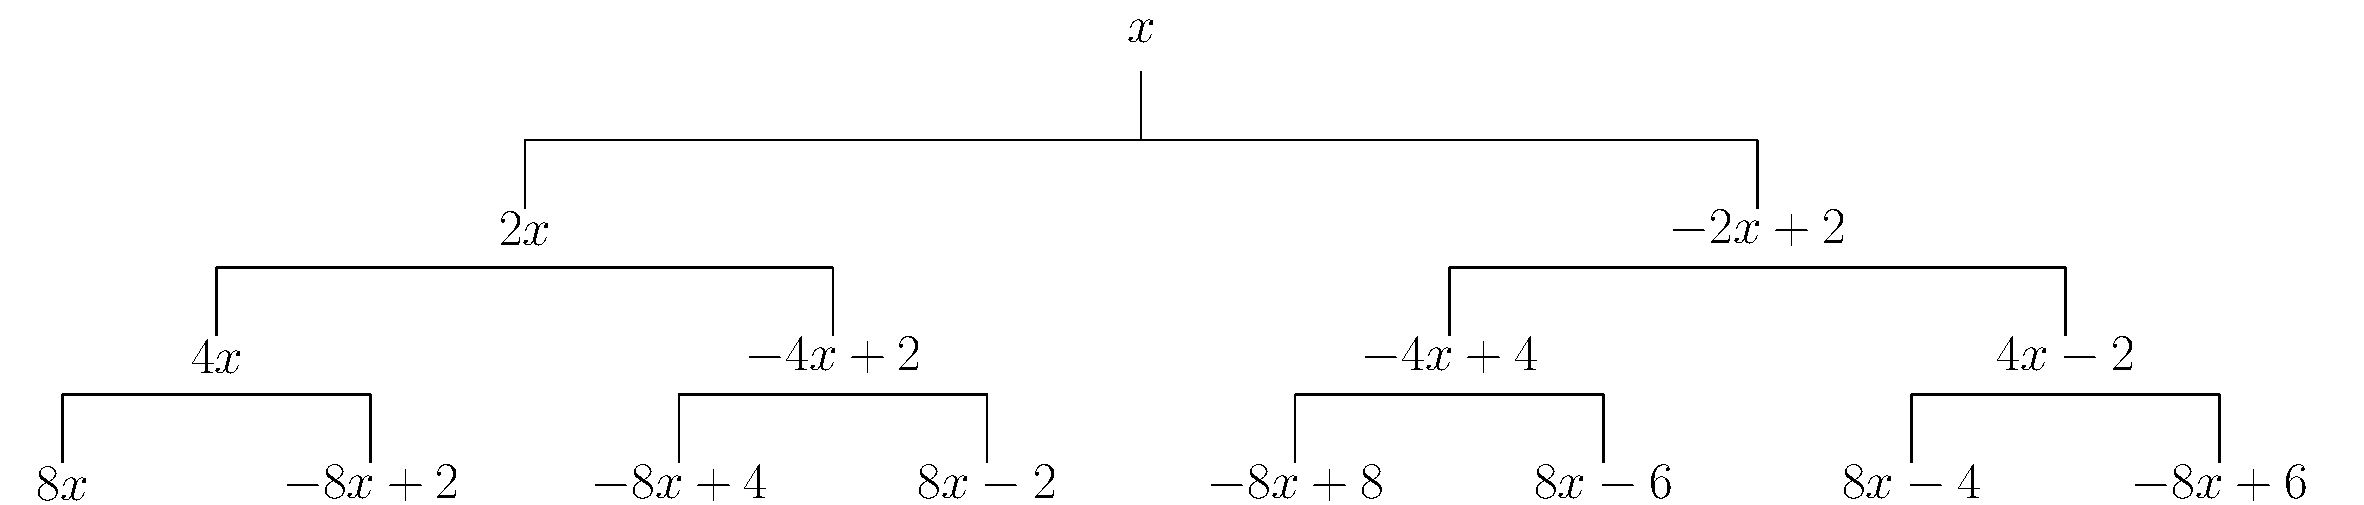
\includegraphics[scale=0.45]{../TeXGraph/Pdf/visuel_2D_arbre_3.pdf}
\captionof{figure}{\emph{L'arbre des positions possibles de $x$ pour $3$ étapes}.}
\end{center}

On remarque que le coefficient de $x$ est une puissance de $2$ dépendante du nombre d'étape. En effet, pour une étape on a $\pm2^1$, pour deux étapes, $\pm2^2$ etc.) De plus, on observe la présence d'une constante entière paire : $-6$, $-4$, $-2$, $0$, $2$, $4$ ou $6$ (pour la troisième étape).

Que faire de ces positions ? Nous pouvons peut-être les trier dans un tableau selon le signe du coefficient de $x$ :

\begin{center}
\begin{tabular}{|c||c|c|}
    \hline
    \multicolumn{2}{|c|}{\textbf{Positions obtenues à la deuxième étape}} \\ \hline\hline
        \multirow{1}{*}{\emph{Coefficient de $x$ négatif}} & \emph{Coefficient de $x$ positif} \\ \hline\hline
        \multirow{1}{*}{$-4x+2$} & $4x-0$ \\ \hline
        \multirow{1}{*}{$-4x+4$} & $4x-2$ \\
    \hline
\end{tabular}
\captionof{figure}{\emph{Tableau des positions obtenues à la deuxième étape selon le signe du coefficient de $x$}.}
\end{center}

De même pour $n=3$ nous construisons un tableau similaire :

\begin{center}
\begin{tabular}{|c||c|c|}
    \hline
    \multicolumn{2}{|c|}{\textbf{Positions obtenues à la troisième étape}} \\ \hline\hline
        \multirow{1}{*}{\emph{Coefficient de $x$ négatif}} & \emph{Coefficient de $x$ positif} \\ \hline\hline
        \multirow{1}{*}{$-8x+2$} & $8x-0$ \\ \hline
        \multirow{1}{*}{$-8x+4$} & $8x-2$ \\ \hline
        \multirow{1}{*}{$-8x+6$} & $8x-4$ \\ \hline
        \multirow{1}{*}{$-8x+8$} & $8x-6$ \\
    \hline
\end{tabular}
\captionof{figure}{\emph{Tableau des positions obtenues à la troisième étape selon le signe du coefficient de $x$}.}
\end{center}

On observe alors une régularité dans la forme de ces positions selon que le coefficient de $x$ soit positif ou négatif. En effet, les positions forment deux groupes dont les termes sont en progression arithmétique\footnote{On rappelle que des entiers sont en progression arithmétique s'il existe un réel $r$ tel que quelque soit deux entiers consécutifs de la progression, leur différence est constante égale à $r$, c'est la \emph{raison}.}.

On émet alors la conjecture :

\newconj{Pour tout entier $n>0$, si $x$ est une position alors les positions possibles\footnote{Si $a\leqslant b$ sont des entiers alors $\left\llbracket a;b\right\rrbracket$ est l'ensemble des entiers compris entre $a$ et $b$.} à l'étape $n$, en partant de $x$, sont :}

\[\left(\textbf{I}\right)\ \ \ \begin{cases}2^nx-2k_1&\text{avec }k_1\in\left\llbracket0;2^{n-1}-1\right\rrbracket\\-2^nx+2k_2&\text{avec }k_2\in\left\llbracket1;2^{n-1}\right\rrbracket\end{cases}\]

\newPreuve{On procède par récurrence :

\begin{enumerate}

\item\textbf{\emph{Initialisation :}} lorsque $n=1$, les positions possibles sont (d'après l'arbre de la figure $5$) : $2x=2^1x+2\times0$ et $-2x+2=-2^1x+2\times1$. Les formules $\left(\textbf{I}\right)$ sont valides à l'étape $1$.
\item\textbf{\emph{Hérédité :}} supposons que les formules $\left(\textbf{I}\right)$ soient valides à l'étape $n$ donc, à l'étape $n+1$ les positions possibles seraient :

\vspace*{-0.25cm}

\begin{center}
\begin{figure}[H]
  \begin{subfigure}[b]{0.4\textwidth}
    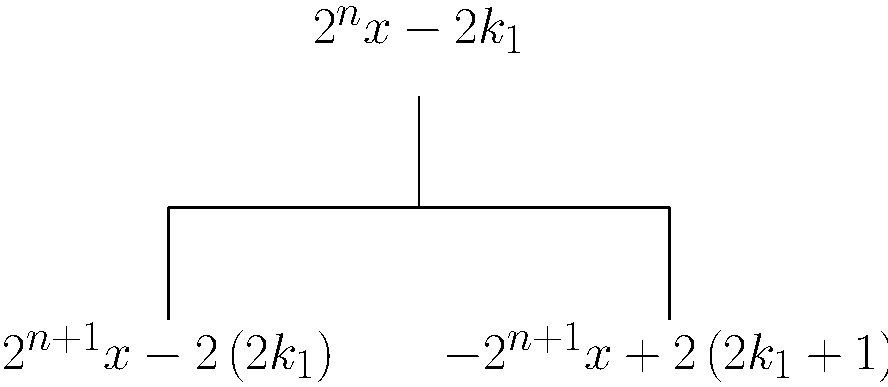
\includegraphics[scale=0.45]{../TeXGraph/Pdf/visuel_2D_arbre_4_part_1.pdf}
    \caption{\emph{Positions possibles avec $2^n$}.}
    \label{fig:f3}
  \end{subfigure}
  \hfill
  \begin{subfigure}[b]{0.4\textwidth}
    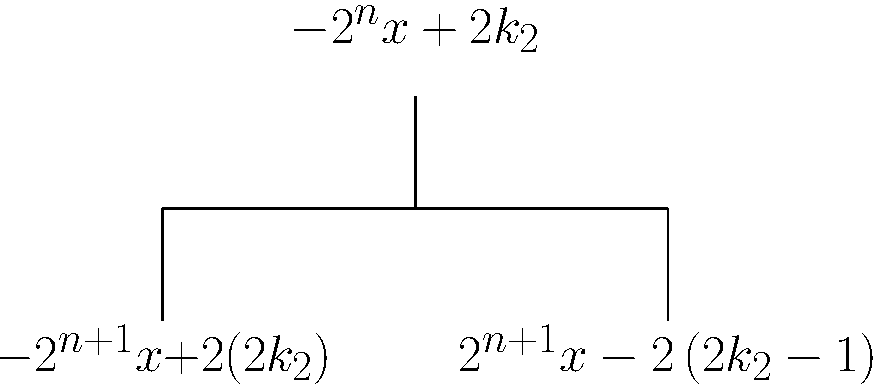
\includegraphics[scale=0.45]{../TeXGraph/Pdf/visuel_2D_arbre_4_part_2.pdf}
    \caption{\emph{Positions possibles avec $-2^n$}.}
    \label{fig:f4}
  \end{subfigure}
  \caption{\emph{Les positions possibles au cas $n+1$}.}
\end{figure}
\end{center}
\vspace*{-1cm}

On remarque que $2k_2-1$ (à gauche de la figure $16$) est l'ensemble des entiers impairs de $1$ à $2^n-1$ (car $k_2$ varie de $1$ à $2^{n-1}$) et que $2k_1$ (à droite) est l'ensemble des entiers pairs de $0$ à $2^n-2$ (car $k_1$ varie de $0$ à $2^{n-1}-1$). 

De plus, $2k_1+1$ (à droite) est l'ensemble des entiers impairs de $1$ à $2^n-1$ et $2k_2$ (à gauche) est l'ensemble des entiers pairs de $2$ à $2^n$. Ainsi, les positions possibles à l'étape $n+1$ sont :
\[\begin{cases}2^{n+1}x-2k_3&\text{avec }k_3\in\left\llbracket0;2^n-1\right\rrbracket\\-2^{n+1}x+2k_4&\text{avec }k_4\in\left\llbracket1;2^n\right\rrbracket\end{cases}\]
car en combinant les expressions $2^{n+1}x-2\left(2k_1\right)$ et $2^{n+1}x-2\left(2k_2-1\right)$ on obtient $2^{n+1}x-2k_3$ où $k_3$ parcourt tous les entiers entre $0$ et $2^n-1$. De même, en combinant les expressions $-2^{n+1}x+2\left(2k_2\right)$ et $-2^{n+1}x+2\left(2k_1+1\right)$ on obtient $-2^{n+1}x+2k_4$ où $k_4$ parcourt tous les entiers entre $1$ et $2^n$.

$\\$
Ainsi, si les formules $\left(\textbf{I}\right)$ sont valides à l'étape $n$ alors elles le sont à l'étape $n+1$. Or elles le sont à l'étape $1$ donc la conjecture est vraie pour tout $n>0$.

$\claim$
\end{enumerate}}

%---------------- Positions périodiques ------------------------------------

\subsection{L'étude des positions périodiques à l'étape $n$}

Dans un second temps, nous allons étudier les positions périodiques à l'étape $n$. Mais avant de les étudier, nous allons trouver leur forme générale grâce à la conjecture $1$.

%---------------- Formule générale ---------------------------------------

\subsubsection{La forme générale de ces positions périodiques}
De la forme générale des positions possible à l'étape $n$ (c.f. \textbf{conjecture $1$}) on en déduit que si $x$ est une position $n$-périodique alors $x=f^n\left(x\right)$ donc l'une des égalités suivantes est vraie :

\[\begin{cases}\left(\textbf{A}\right)\ \ \ x=2^nx-2k_1&\text{avec }k_1\in\left\llbracket0;2^n-1\right\rrbracket\\\left(\textbf{B}\right)\ \ \ x=-2^nx+2k_2&\text{avec }k_2\in\left\llbracket1;2^n\right\rrbracket\end{cases}\]

En résolvant l'égalité $\left(\textbf{A}\right)$ on a :

\[x=2^nx-2k_1\Longleftrightarrow x\left(1-2^n\right)=-2k_1\Longleftrightarrow x=\frac{2k_1}{2^n-1}\text{ avec }k_1\in\left\llbracket0;2^{n-1}-1\right\rrbracket\]

De même avec $\left(\textbf{B}\right)$ :

\[x=-2^nx+2k_2\Longleftrightarrow x\left(1+2^n\right)=2k_2\Longleftrightarrow x=\frac{2k_2}{2^n+1}\text{ avec }k_2\in\left\llbracket1;2^{n-1}\right\rrbracket\]

Ainsi, l'ensemble des positions $n$-périodiques est donné par :
\[\left(\textbf{II}\right)\ \ \ \begin{cases}x=\frac{2k_1}{2^n-1}\text{ avec }k_1\in\left\llbracket0;2^{n-1}-1\right\rrbracket\\x=\frac{2k_2}{2^n+1}\text{ avec }k_2\in\left\llbracket1;2^{n-1}\right\rrbracket\end{cases}\]

Nous résumons quelques solutions de $\left(\textbf{II}\right)$ par un tableau :
\begin{center}
\begin{tabular}{|c||c|c|}
    \hline
    \multicolumn{3}{|c|}{\textbf{Positions périodiques pour un petit nombre d'étapes}} \\ \hline\hline
        \multirow{1}{*}{\emph{Étape}} & \emph{Ensemble des positions périodiques} & \emph{Nombre de positions périodiques} \\ \hline\hline
        \multirow{1}{*}{$1$} & $\left\{0;\frac{2}{3}\right\}$ & $2^1$ \\ \hline
        \multirow{1}{*}{$2$} & $\left\{0;\frac{2}{3};\frac{2}{5};\frac{4}{5}\right\}$ & $4=2^2$ \\ \hline
        \multirow{1}{*}{$3$} & $\left\{0;\frac{2}{7};\frac{4}{7};\frac{6}{7};\frac{2}{9};\frac{4}{9};\frac{6}{9};\frac{8}{9}\right\}$ & $8=2^3$ \\ \hline
        \multirow{1}{*}{$4$} & $\left\{0;\frac{2}{15};\frac{4}{15};\frac{6}{15};\frac{8}{15};\frac{10}{15};\frac{12}{15};\frac{14}{15};\frac{2}{17};\frac{4}{17};\frac{6}{17};\frac{8}{17};\frac{10}{17};\frac{12}{17};\frac{14}{17};\frac{16}{17}\right\}$ & $16=2^4$ \\
    \hline
\end{tabular}
\captionof{figure}{\emph{Résumé des positions périodiques pour un nombre d'étapes allant de $1$ à $4$}.}
\end{center}

Nous voyons que le nombre de positions $n$-périodiques croit au fur et à mesure des étapes. Mais combien y a-t-il de positions $n$-périodiques ?

%---------------- Nombre de solutions ------------------------------------

\subsubsection{Le nombre de positions périodiques à l'étape $n$}
D'après le tableau figure $20$ il semblerait que le nombre de positions $n$-périodiques distinctes soit de $2^n$. On conjecture alors :

\newconj{Soit un entier $n>0$, il y a exactement $2^n$ positions $n$-périodiques distinctes.}

\newPreuve{Par l'absurde, supposons qu'il existe deux positions $n$-périodiques égales avec des numérateurs distincts. Si leurs dénominateurs sont distincts (donc de la forme $2^n-1$ et $2^n+1$) alors puisque $\operatorname{PGCD}\left(2^n-1;2^n+1\right)=1$ ces positions, dans leur forme irréductible, auront des dénominateurs distincts. Donc elles ne peuvent être égales car si deux fractions sont égales alors elles ont la même forme irréductible. De même, si elles ont des dénominateurs égaux, alors leur numérateurs le sont aussi, contradiction.}

Nous allons maintenant passer à l'étude de ces positions périodiques notamment grâce à l'étude des cycles qu'elles forment.

%---------------- Positions n-périodiques ------------------------------------

\subsection{L'étude des positions $n$-périodiques}
Dans cette partie, nous étudierons quelques propriétés des positions $n$-périodiques. Nous verrons tout d'abord un lemme utile qui nous permettra de trouver une formule pour énumérer les positions qui se répètent pour la première fois à l'étape $n$. Nous finirons cette partie en évoquant un célèbre théorème, le petit théorème de Fermat\footnote{\href{https://fr.wikipedia.org/wiki/Pierre_de_Fermat}{\emph{Pierre de Fermat}} (début $XVII$ - 1665), mathématicien français, il est surtout connu d'avoir énoncé le dernier théorème de Fermat, une conjecture récemment démontrée.}.
\subsubsection{Un lemme sur les diviseurs}
Dans un premier temps on définie une fonction $\operatorname{P}$ :

\newDef{Soit $\operatorname{P} : \left[0;1\right]\to\mathbb{N}^*$ la fonction qui à toute position périodique $x$ associe le plus petit entier naturel non nul $n$ tel que $f^n\left(x\right)=x$, on note $\operatorname{P}\left(x\right)=n$.}

Nous dirons qu'une telle position périodique $x$ est exactement $n$-périodique.

On arrive alors au lemme :

\hypertarget{18}{}
\newlemme{Soit $x$ une position périodique et $n$ un entier naturel alors $f^n\left(x\right)=x$ si et seulement si $\operatorname{P}\left(x\right)|n$}

\newPreuve{On démontre d'abord que si $\operatorname{P}\left(x\right)|n$ alors $f^n\left(x\right)=x$. Si $\operatorname{P}\left(x\right)|n$ alors il existe un entier relatif $m$ tel que $m\operatorname{P}\left(x\right)=n$ donc $f^n\left(x\right)=f^{m\operatorname{P}\left(x\right)}\left(x\right)=\underbrace{f^{\operatorname{P}\left(x\right)}\left(f^{\operatorname{P}\left(x\right)}\left(\ldots f^{\operatorname{P}\left(x\right)}\left(x\right)\ldots\right)\right)}_{m\text{ fois}}=x$

Maintenant on démontre que si $f^n\left(x\right)=x$ alors $\operatorname{P}\left(x\right)|n$. D'après la \hyperlink{15}{\textbf{propriété 1}} il existe des entiers naturels $q$ et $0\leqslant r<\operatorname{P}\left(x\right)$ tel que $n=q\operatorname{P}\left(x\right)+r$. Donc $f^n\left(x\right)=f^{q\operatorname{P}\left(x\right)+r}\left(x\right)=f^r\left(\underbrace{f^{\operatorname{P}\left(x\right)}\left(\ldots f^{\operatorname{P}\left(x\right)}\left(x\right)\ldots\right)}_{q\text{ fois}}\right)=f^r\left(x\right)=x$ or $r<\operatorname{P}\left(x\right)$ donc d'après la définition de $\operatorname{P}$, si $r>0$ alors $\operatorname{P}\left(x\right)\leqslant r$ mais c'est absurde, donc on a $r=0$ d'où $\operatorname{P}\left(x\right)|n$.}

Penchons-nous maintenant sur la question : \emph{combien existe t-il de positions telles que la coquille revienne pour la première fois à sa position initiale après $n$ étapes ?} On pose la définition :

\newDef{Soit $\operatorname{S} : \mathbb{N}^*\to\mathbb{N}^*$ la fonction qui à tout entier naturel non nul $n$ associe le nombre de positions périodiques $x$ telles que $\operatorname{P}\left(x\right)=n$.}

D'après le \hyperlink{18}{\textbf{lemme 1}} il suit que les positions qui se répètent au bout de $n$ étapes sont des positions $x$ telles que $\operatorname{P}\left(x\right)|n$ et elles sont au nombre de $2^n$. Ainsi, si nous voulons seulement les positions $x$ telles que $\operatorname{P}\left(x\right)=n$ il faut soustraire à $2^n$ le nombre de positions $x$ qui satisfont\footnote{On dira que $\operatorname{P}\left(x\right)$ est un diviseur strict de $n$.} $\operatorname{P}\left(x\right)<n$ et $\operatorname{P}\left(x\right)|n$. 

Par exemple pour un nombre premier, comme $5$, il faut seulement enlever les positions qui reviennent à chaque étape (car $1$ est le seul diviseur strict positif de $5$) ainsi $\operatorname{S}\left(5\right)=2^5-\operatorname{S}\left(1\right)=32-2=30$ car $\operatorname{S}\left(1\right)=2$ puisque $0$ et $\frac{2}{3}$ sont les seules positions $1$-périodiques.

De même pour $10$, ses diviseurs stricts positifs sont élément de $\left\{1;2;5\right\}$ donc $\operatorname{S}\left(10\right)=2^{10}-\operatorname{S}\left(5\right)-\operatorname{S}\left(2\right)-\operatorname{S}\left(1\right)=1024-30-\left(2^2-\operatorname{S}\left(1\right)\right)-2=990$.

Dans la partie suivante, nous allons trouver une formule récurrente pour calculer explicitement la valeur de $\operatorname{S}\left(n\right)$ pour $n\in\mathbb{N}$.

\hypertarget{50}{}
\subsubsection{Une forme récurrente pour $\operatorname{S}$}
Les calculs précédents de $\operatorname{S}\left(5\right)$ et de $\operatorname{S}\left(10\right)$ mettent en exergue une certaine manière de calculer $\operatorname{S}\left(n\right)$ pour $n\in\mathbb{N}^*$. En effet, puisque $\operatorname{S}\left(n\right)$ représente le nombre de positions $x\in\left[0;1\right]$, périodiques, vérifiant $\operatorname{P}\left(x\right)=n$ et qu'il y a au total $2^n$ positions $n$-périodiques alors il suffit de retirer, pour chaque diviseur strict positif $d$ de $n$, $\operatorname{S}\left(d\right)$ à $2^n$. En effet, les ensembles formés par les positions exactement $d$-périodiques sont mutuellement disjoints et sont sous-ensembles de l'ensemble des positions $n$-périodique. De cette analogie avec les ensembles on en déduit une égalité sur leur cardinal i.e. : 
\[\operatorname{S}\left(n\right)=2^n-\sum_{\substack{d|n\\0<d<n}}\operatorname{S}\left(d\right)\]
c'est la formule de récurrence.


\subsubsection{Calcul de $\operatorname{S}\left(n\right)$ pour $n\in\mathbb{N}$}

Comme nous l'avons vu précédemment, pour calculer $\operatorname{S}\left(n\right)$ avec $n\in\mathbb{N}$ nous devons soustraire à $2^n$ la somme des $\operatorname{S}\left(d\right)$ où $d$ est un diviseur strict positif de $n$. Voici dans un premier temps un algorithme qui calcul $\operatorname{S}\left(n\right)$ :

\begin{center}
\begin{minted}[frame=lines,breaklines,framesep=12pt,baselinestretch=1.2,bgcolor=bg,fontsize=\footnotesize,linenos]{text}
Définir un dictionnaire, # Pour éviter de recalculer certaines valeurs.
Définir une fonction récurrente de paramètre n (un entier naturel),
Définir le résultat S et y stocker 2**n,
Pour chaque diviseur strict positif d de n :
    Si on connaît déjà S(d) :
        Mettre S à S-S(d),
    Sinon :
        Ré-appeler la fonction avec comme paramètre d,
        Stocker dans le dictionnaire la couple clé-valeur (d,S(d)),
        Mettre S à S-S(d),
Retourner S
\end{minted}
\captionof{figure}{\emph{Algorithme de calcul de $\operatorname{S}\left(n\right)$}.}
\end{center}

Le dictionnaire de la ligne $1$ stocke les valeurs calculées comme des couples $\left(\text{clé};\text{valeur}\right)$ et dans notre cas \emph{clé} correspond à l'entier naturel $n$ et la \emph{valeur} à $\operatorname{S}\left(n\right)$. De cet algorithme on construit notre programme (en Python) :
    
\begin{center}
\begin{minted}[frame=lines,breaklines,framesep=12pt,baselinestretch=1.2,bgcolor=bg,fontsize=\footnotesize,linenos]{python}
from sympy import divisors

d={1:2}  # Contient : 'clé' (le nombre d'étape, 'n') et 'valeur' (nombre de solutions d'orbite 'n').
def S_n(n):
    '''Fonction récurrente pour obtenir le nombre de solutions d'orbite 'n'.'''
    S=2**n  # Le nombre de solutions de période divisant 'n'.
    for diviseur in divisors(n)[:-1]:  # On parcourt la liste des diviseurs de 'n' sauf 'n'.
        v=d.get(diviseur,0)
        if v:  # Si on connaît le nombre de solutions d'orbite 'diviseur'.
            S-=v  # On le soustrait à 'S'.
        else:  # Sinon on le calcul, on l'ajoute au dictionnaire puis on le soustrait.
            v=S_n(diviseur)
            d[diviseur]=v
            S-=v
    return S
\end{minted}
\captionof{figure}{\emph{Code source du programme Python}.}
\end{center}

Nous utilisons la fonction \emph{divisors} du module \emph{sympy} (ligne $1$). Cette fonction, d'une part calcule les diviseurs positifs d'un entier naturel et, d'autre part elle est \emph{très} optimisée. Comme nous calculons à de nombreuses reprises les diviseurs de $n$ (et même si nous les stockons dans un dictionnaire, voir la ligne $3$) il est nécessaire que cette fonction soit rapide.

\subsubsection{Formule explicite de $\operatorname{S}\left(n\right)$}

Notez aussi que la fonction $\operatorname{S}\left(n\right)$ peut se calculer explicitement à l'aide des diviseurs de $n$. En reprenant la relation de récurrence trouvée en \hyperlink{50}{\textbf{$2$.$3$.$2$}},

\begin{align*}
\operatorname{S}\left(n\right)&=2^{n}-\sum_{\substack{d_{1}|n \\ 0<d_{1}<n}}\operatorname{S}\left(d_{1}\right)\\
&=2^{n}-\sum_{\substack{d_{1}|n \\ 0<d_{1}<n}}\left(2^{d_{1}}-\sum_{\substack{d_{2}|d_{1}\\0<d_{2}<d_{1}<n}}\operatorname{S}\left(d_{2}\right)\right)\\
&=2^{n}-\sum_{\substack{d_{1}|n \\ 0<d_{1}<n}}2^{d_{1}}+\sum_{\substack{d_{2}|d_{1}, d_{1}|n\\0<d_{2}<d_{1}<n}}\operatorname{S}\left(d_{2}\right)\\
\end{align*}

On voit alors se dessiner la formule générale,
\[\operatorname{S}\left(n\right)=2^{n}-\sum_{k\in\mathbb{N}^*}\left(\left(-1\right)^{k+1}\times\sum_{\substack{d_{k}|d_{k-1},\ldots, d_{2}|d_{1},d_{1}|n\\ 0<d_{k}<d_{k-1}<\ldots<d_{2}<d_{1}<n}}2^{d_{k}}\right)\]
où $k$ parcourt les entier naturels non-nul. Évidemment $k$ ne peut croître indéfiniement et (naïvement), un majorant\footnote{On peut réduire ce majorant à $\tau\left(n\right)-1$, le nombre de diviseurs stricts positifs de $n$ (la présence du $-1$ signal le retrait d'un diviseur positif, ici $n$).} de $k$ est $n-1$ car il y a $n-1$ entiers strictement compris entre $0$ et $n$.

Il est toutefois intéressant de remarquer que $\operatorname{S}\left(n\right)$ peut s'exprimer comme une somme de puissances de $2$. D'ailleurs, on peut établir une analogie entre la formule du crible de Poincaré et la formule ci-dessus.

\subsubsection{Une propriété de $\operatorname{S}$ et le petit théorème de Fermat}

Lorsque $n$ est un nombre premier, ses diviseurs positifs sont $1$ et $n$ donc $\operatorname{S}\left(n\right)=2^{n}-2$ d'après les formules précédentes. Or, il se trouve que quel que soit l'entier $n$ premier, $2^n - 2$ est divisible par $n$.

Pour le démontrer, supposons que l'on ait trouvé une position, disons $k_{1}$, qui revienne pour la première fois au bout de $n$ étapes (on rappelle que $n$ est premier). Ainsi, $\operatorname{P}\left(k_{1}\right)=n$. Schématiquement on a :

\begin{center}
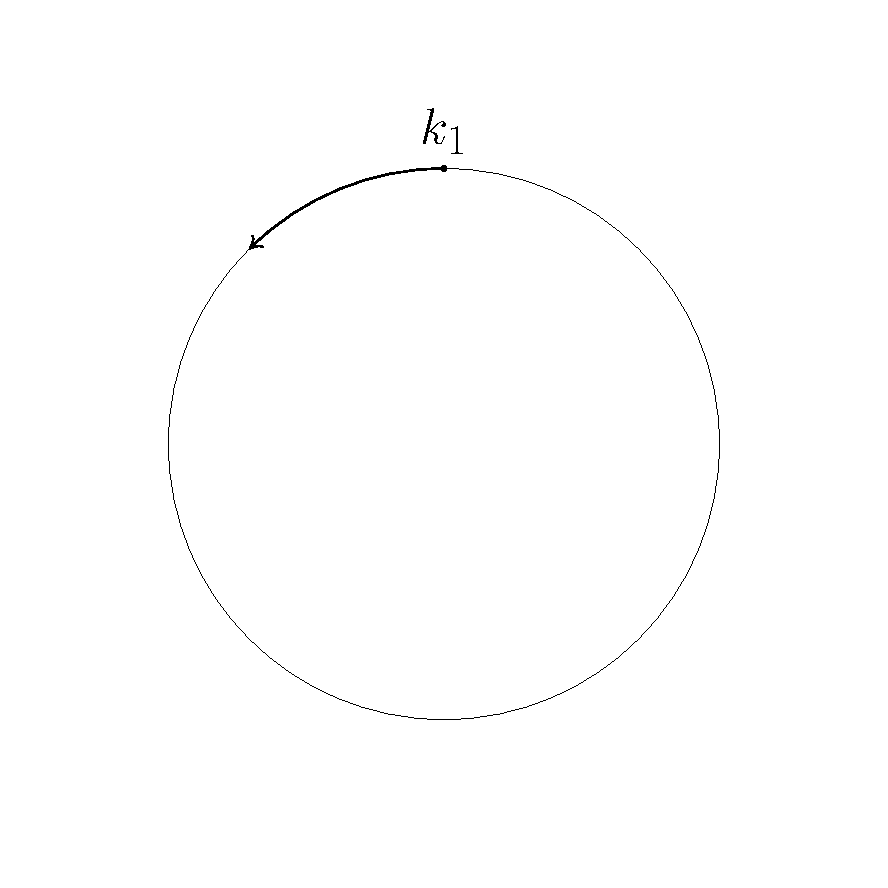
\includegraphics[scale=0.45]{../TeXGraph/Pdf/position_periodique_1.pdf}
\captionof{figure}{\emph{Shéma du cycle des positions}.}
\end{center}

Cette position va former un cycle de taille $n$ donc la coquille aura, disons, pour positions $k_2$ puis $k_3$, $\ldots$, $k_n$,

\begin{center}
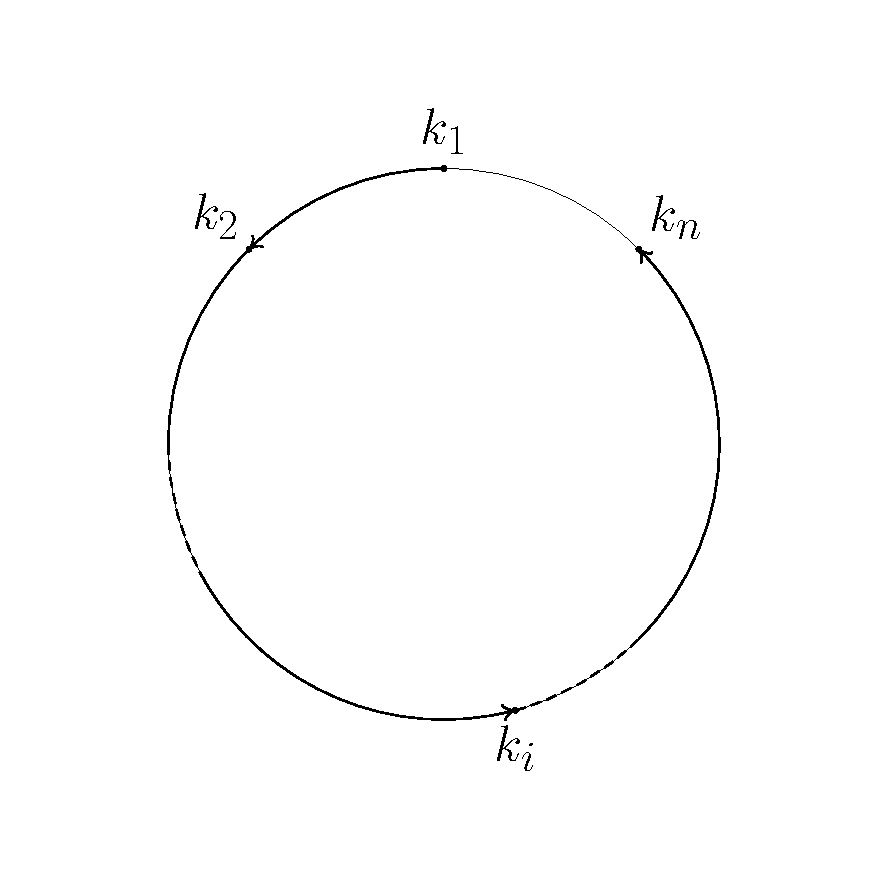
\includegraphics[scale=0.45]{../TeXGraph/Pdf/position_periodique_2.pdf}
\captionof{figure}{\emph{Shéma du cycle des positions}.}
\end{center}

Maintenant, si au lieu de choisir $k_1$ comme position initiale on choisit la suivante soit $k_2$, alors elle aussi retrouvera sa position pour la première fois dans $n$ étapes : $k_2\rightarrow k_3\rightarrow\ldots\rightarrow k_n\rightarrow k_1\rightarrow k_2$ et ainsi de suite. On montre bien que pour chaque solution trouvée il en existe $n-1$ autres. Ainsi, on forme des paquets de $n$ solutions et comme il y en a $2^n - 2$ on en déduit que $2^n - 2$ est un multiple de $n$.


Et on peut généraliser. En effet, supposons que l'on étale notre pâte, non pas en deux, mais en $a$ parts (toutes égales) puis que l'on rabat successivement les $a$ parties sur elles-mêmes en commençant par la partie la plus \emph{haute}. Ainsi, notre arbre sera constitué, non pas de $2^n$ mais, de $a^n$ branches au bout de $n$ étapes (avec $n$ un entier naturel non-nul). Pour un entier naturel $n$ premier il y aura donc $a^n - a$ solutions. Et le même raisonnement s'applique, on en déduit donc que, quel que soit l'entier naturel $a\geqslant 2$ et quel que soit l'entier naturel $n$ premier, $a^n - a$ est un multiple de $n$. 

Ce résultat est un théorème célèbre : le petit théorème de Fermat (que l'on démontre traditionnellement par induction). Si $p$ est un nombre premier et $a$ un entier,
\[a^p-a\equiv0\pmod{p}\]
et si $p$ ne divise pas $a$,
\[a^{p-1}-1\equiv0\pmod{p}\]

\hypertarget{1}{}
\subsection{L'étude des positions non périodiques}
Après avoir approfondi l'existence de positions périodiques, voyons ce qu'il en est des positions non périodiques. Nous scindons cette \emph{étude} en deux parties : une étude sur les positions rationnelles et une autre sur les positions irrationnelles.
\subsubsection{Chez les rationnels}
Chez les rationnels, l'étude des positions périodiques montre que seules les positions de la forme :
\[\begin{cases}x=\frac{2k_1}{2^n-1}\text{ avec }k_1\in\left\llbracket0;2^{n-1}-1\right\rrbracket\\x=\frac{2k_2}{2^n+1}\text{ avec }k_2\in\left\llbracket1;2^{n-1}\right\rrbracket\end{cases}\]
le sont, pour tout entier naturel non nul $n$. Ainsi, les positions $\frac{1}{3}$, $\frac{1}{11}$ ou même $\frac{7}{8}$ ne pouvant être exprimées sous la forme ci-dessus ne sont donc pas périodiques. On peut d'ailleurs remarquer qu'une condition nécessaire pour la périodicité d'une position est que, sous forme irréductible, celle-ci doit avoir un numérateur pair. Cette remarque découle de $\operatorname{PGCD}\left(2^n\pm1;2\right)=1$ pour tout entier $n>0$.

Mais on remarque le phénomène :
\[\begin{cases}f\left(\frac{1}{3}\right)=\frac{2}{3}\\f^4\left(\frac{7}{8}\right)=f^3\left(\frac{2}{8}\right)=f^2\left(\frac{4}{8}\right)=f\left(\frac{8}{8}\right)=0\end{cases}\]
Il semblerait donc que toutes positions rationnelles non périodiques mène à un cycle.

\newconj{Si $x$ est une position rationnelle non périodique alors il existe un entier $k$ tel que $f^k\left(x\right)$ soit une position périodique.}

\newPreuve{Puisque $x$ est une position rationnelle alors il existe deux entiers $0<p\leqslant q$ tels que $x=\frac{p}{q}$. On remarque aussi que la transformation du boulanger sur $x$ n'affecte que le numérateur, en effet $f\left(x\right)=\frac{q-\left\lvert2p-q\right\rvert}{q}$. Soit $E$, l'ensemble des numérateurs que prend successivement $x$ jusqu'à la $q-1$-ème étape (incluse). Donc $E$ contient $q$ entiers de l'intervalle $\left\llbracket1;q\right\rrbracket$ (qui sont $p$, $qf\left(x\right)$, $qf^2\left(x\right)\ldots qf^{q-1}\left(x\right)$). Or $0<p\leqslant q$ donc $p$ ne peut prendre que $q-1$ valeurs différentes ($1$, $2\ldots q$) ainsi, d'après le principe des tiroirs deux valeurs de $E$ sont égales, on a donc un cycle.}

Finalement, nous avons vu que même si une position non périodique est rationnelle, celle-ci mènera à une position périodique. Ceci est loin d'être la cas pour les nombres irrationnels.
\subsubsection{Chez les irrationnels}
Nous savons qu'un nombre est irrationnel s'il ne peut être exprimé comme un quotient deux entiers. Par exemple, $\sqrt{2}-1$ ou $\sqrt{3}-1$ sont des nombres irrationnels (en l'occurrence, des positions irrationnelles). Nous avons conjecturé au vu du \hyperlink{4}{graphique $13\ (b)$} que toute les positions irrationnelles sont non périodiques. Ceci découle en partie du fait que d'après la forme générale des positions périodiques, celles-ci sont toutes rationnelles.

\newconj{Aucune position irrationnelle n'est périodique.}

\newPreuve{Soit $x$ une position irrationnelle ($x\in\left[0;1\right]$ et $x\not\in\mathbb{Q}$), on démontre par l'absurde que $f\left(x\right)$ est irrationnelle. En effet, si $x\leqslant\frac{1}{2}$ alors $f\left(x\right)=2x$. Si $2x$ est rationnel alors on a $2x=\frac{p}{q}$ pour des entiers $p$ et $q\not=0$, d'où $x=\frac{p}{2q}$, ce qui est contradictoire, donc $2x$ est irrationnel. De même, si $x>\frac{1}{2}$ alors $f\left(x\right)=2-2x$ et si $2-2x$ est rationnel alors on a $2-2x=\frac{p}{q}$ pour des entiers $p$ et $q\not=0$ d'où $x=\frac{2q-p}{2q}$, absurde donc $2-2x$ est irrationnel. On conclut donc que si $x$ est irrationnel alors $f\left(x\right)$ l'est aussi et, récursivement $f^k\left(x\right)$ est irrationnel pour tout entier naturel $k$.}

\section{L'approche binaire}
Notre chercheur nous a conseillé aussi d'aborder le problème sous une autre base de nombre, la base $2$. Cette approche s'est révélée fructueuse pour notre problème.

Dans un premier temps, nous allons apprendre à convertir les rationnels positifs\footnote{Les éléments de $\mathbb{Q}_+$.} de base $10$ à base $2$ puis, nous verrons les avantages de la base $2$ et finalement, nous étudierons les positions périodique.
\subsection{Le passage de base $10$ à base $2$, une généralité}
\subsubsection{Chez les entiers positifs}
Tout d'abord nous introduisons un théorème fondamental, le théorème de la division euclidienne (nous nous concentrerons exclusivement sur les entiers positifs) :

\hypertarget{15}{}
\newprop{Pour tout couple d'entiers positifs $\left(a;b\right)$ avec $b>0$ il existe un unique couple d'entiers positifs $\left(q;r\right)$ tel que $a=bq+r$ et $r<b$.}

\newPreuve Pour l'existence d'un couple $\left(q;r\right)$ d'entiers positifs, on prend $q$ le plus grand entier tel que $bq\leqslant a<b\left(q+1\right)$ et on a $r=a-bq$ et il vérifie $0\leqslant r<b\left(q+1\right)-bq=b$.

Pour l'unicité, on suppose qu'il existe deux couples d'entiers positifs $\left(q_0;r_0\right)$ et $\left(q_1;r_1\right)$ tel que $a=bq_0+r_0=bq_1+r_1$ avec $r_0<b$ et $r_1<b$. Ainsi, $b\left(q_0-q_1\right)=r_1-r_0$ donc $b|\left(r_1-r_0\right)$ or $b>r_1-r_0$, on en déduit $r_0=r_1$. Finalement on obtient $bq_0=bq_1$ et puisque $b>0$ on abouti à $q_0=q_1$ en divisant par $b$ de chaque côté.

De cette proposition découle le corollaire\footnote{Un corollaire est un résultat qui se déduit d'un résultat précédent.} :

\newcoro{Pour tout couple d'entiers positifs $\left(a;b\right)$ avec $b>1$ il existe un unique $n$-uplet d'entiers positifs $\left(r_0,r_1,\ldots,r_{n-1}\right)$ de $\left\llbracket0;b\right\llbracket^n$ tel que $a=b^{n-1}r_{n-1}+b^{n-2}r_{n-2}+\ldots+br_1+r_0$.}

\newPreuve L'existence et l'unicité d'un tel $n$-uplet d'entiers de $\left\llbracket0;b\right\llbracket^n$ se déduit de la division euclidienne de $a$ par $b$. En effet, il existe un unique couple d'entiers $\left(q_0;r_0\right)$ tel que $a=bq_0+r_0$ et $r_0\in\left\llbracket0;b\right\llbracket$. De même il existe un unique couple d'entiers $\left(q_1;r_1\right)$ avec $r_1\in\left\llbracket0;b\right\llbracket$ tel que $q_0=bq_1+r_1$ ainsi, $a=b^2q_1+br_1+r_0$. Tant que les quotient sont strictement positifs on continue à les diviser par $b$ et du fait que $b>1$ on a $a>q_0>q_1>\ldots>q_{n-2}$ avec $0<q_{n-2}<b$ pour un entier positif $n$. De là, $q_{n-2}=b\times0+r_{n-1}$. On construit alors des entiers $r_0,r_1,\ldots,r_{n-1}$ de $\left\llbracket0;b\right\llbracket$ qui satisfont $a=b^{n-1}r_{n-1}+b^{n-2}r_{n-2}+\ldots br_1+r_0$ et ils sont uniques car les couples $\left(q_0;r_0\right),\left(q_1;r_1\right),\ldots,\left(q_{n-1};r_{n-1}\right)$ le sont d'après la proposition ci-dessus.

\textbf{Remarques} : 
\begin{enumerate}
\item Pour plus de lisibilité on note $a=\overline{r_{n-1}r_{n-2}\ldots r_1r_0}^{\left(b\right)}$ la représentation de $a$ en base $b$.
\item Multiplier $a$ par $b$ revient à ajouter $0$ au chiffre des unités de $a$ and base $b$ i.e. $ab=\overline{r_{n-1}r_{n-2}\ldots r_1r_00}^{\left(b\right)}$.
\end{enumerate}

\subsubsection{Chez les rationnels positifs}
Il est possible d'étendre la représentation des entiers positifs en base $b$ aux rationnels positifs en base $b$. Nous admettrons la propriété :

\hypertarget{5}{}
\newprop{Pour tout réel $0<r<1$ il existe des entiers $r_1,r_2,r_3\ldots\in\{0;1\}$ tels que $r=\frac{r_1}{2}+\frac{r_2}{2^2}+\frac{r_3}{2^3}+\ldots$ Le nombre $\overline{0{,}r_1r_2r_3\ldots}^{\left(2\right)}$ représente $r$ en base $2$.}

Par exemple, $\frac{2}{3}=\overline{0{,}10\ldots}^{\left(2\right)}$ et $\frac{2}{5}=\overline{0{,}0110\ldots}^{\left(2\right)}$, ici, les blocs $10$ et $0110$ se répètent indéfiniment\footnote{Dans ce qui suit la mention «$\ldots$» dans l'écriture binaire signifiera que les blocs de chiffres (de la virgule jusqu'à «$\ldots$») se répètent indéfiniment.}. 

Nous avons écrit un algorithme qui, pour un nombre une position rationnelle donnée renvoie son écriture en base $2$. Comme pour le \hyperlink{6}{programme précédent}, nous ne nous intéressons qu'aux positions rationnelles et nous séparons numérateur et dénominateur :

\begin{center}
\begin{minted}[frame=lines,breaklines,framesep=12pt,baselinestretch=1.2,bgcolor=bg,fontsize=\footnotesize,linenos]{text}
Définir une position rationnelle,
Définir une précision (le nombre de chiffres à calculer),
Définir 'unité' (le chiffre des unités de la position) et le mettre à 0,
Définir la chaîne de caractère 'binaire',
Tant qu'il reste des chiffres à calculer :
    Doubler le numérateur,
    Si le numérateur est supérieur ou égal au dénominateur : 
        Mettre 'unité' à 1,
    Sinon :
        Mettre 'unité' à 0,
    Ajouter 'unité' à la chaîne 'binaire',
    Soustraire le dénominateur au numérateur si 'unité' vaut 1,
Afficher 'binaire'.
\end{minted}
\captionof{figure}{\emph{Algorithme pour passer de base $10$ à base $2$}.}
\end{center}

D'après la propriété \hyperlink{5}{ci-dessus}, lorsque nous multiplions $r$ par $2$ cela revient à décaler la virgule d'un cran vers la droite dans le représentation de $r$ en base $2$. Donc, si $r=\overline{0,r_1r_2r_3\ldots}^{\left(2\right)}$ alors $2r=\overline{r_1,r_2r_3\ldots}^{\left(2\right)}$. Ainsi, nous multiplions le numérateur par $2$ (ligne $6$), puis nous récupérons le chiffre des unités (d'abord $r_1$ puis $r_2$...) aux lignes $7-8-9-10$. Enfin, on ajoute le chiffre des unités à la chaîne \emph{binaire} (ligne $11$) sans oublier de soustraire le numérateur par le dénominateur si celui-ci est supérieur au dénominateur. De cet algorithme on construit notre programme (en Python) :

\begin{center}
\begin{minted}[frame=lines,breaklines,framesep=12pt,baselinestretch=1.2,bgcolor=bg,fontsize=\footnotesize,linenos]{python}
def binaire(num,den,precision=1000):
    '''Converti une position "num/den" en binaire.'''
    binaire="" # Résultat en binaire.
    unite=0 # Chiffre des unité de la position.
    for k in range(precision): # On calcul 'precision' chiffres après la virgule.
        num*=2
        if num>=den: unite=1 # Si 'num/den' a pour chiffre des unités 1.
        else: unite=0 # Sinon 'num/den' a pour chiffre des unités 0.
        binaire+=str(unite) # On ajoute ce chiffre des unités.
        num-=den*unite # On soustrait le dénominateur au numérateur si 'unité' vaut 1.
    # On renvoie le nombre en binaire avec 'precision' chiffres après la virgule.
    return binaire
\end{minted}
\captionof{figure}{\emph{Code source du programme Python}.}
\end{center}

À la ligne $10$, si le numérateur est inférieur au dénominateur alors la variable \emph{unité} vaut $0$ donc on ne soustrait rien au numérateur. Au contraire, si la variable \emph{unité} vaut $1$ alors on soustrait le dénominateur au numérateur comme voulu.

\subsection{Les avantages du binaire}
\subsubsection{Une nouvelle façon de voir la pâte feuilletée}
Puisque toute position à une représentation en base $2$, nous pouvons re-dessiner la pâte feuilletée de manière à l'adapter à la base $2$ :

\begin{center}
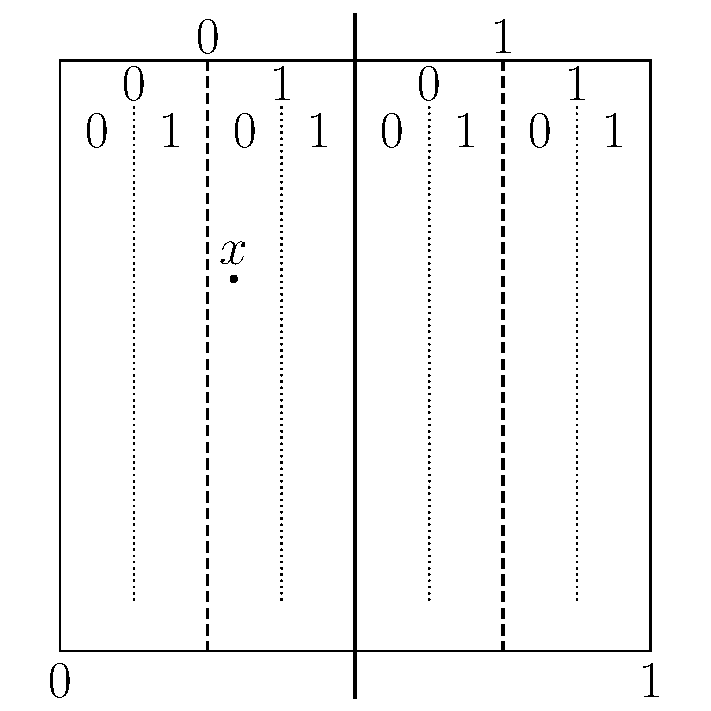
\includegraphics[scale=0.45]{../TeXGraph/Pdf/visuel_2D_pate_binaire.pdf}
\captionof{figure}{\emph{Un nouveau point de vue sur la pâte feuilletée}.}
\end{center}

Cette nouvelle vision de la pâte feuilletée, plus adaptée pour l'approche binaire, permet de cerner plus rapidement la représentation binaire d'une position. Par exemple la représentation en base $2$ de la position $x$ ci-dessus commencerait par $\overline{0{,}010\ldots}^{\left(2\right)}$. Pour continuer ce schéma, il suffit de prend un des $8$ rectangles, de le découper en deux partie \emph{égales}, de numéroté la partie de gauche par un $0$ et celle de droite par un $1$.

De plus, ce schéma permet de savoir dans quelles partie de la pâte feuilletée se trouvera $x$ après un nombre donné (relativement court\footnote{Plus le nombre d'étape est important plus il faudra un encadrement précis de $x$ au départ. Par exemple, si $\frac{1}{8}<x<\frac{3}{8}$ alors $\frac{1}{4}<2x<\frac{3}{4}$ mais $\frac{3}{8}-\frac{1}{8}=\frac{1}{4}<\frac{3}{4}-\frac{1}{4}=\frac{1}{2}$.}) d'étapes. Par exemple, puisque $x=\overline{0{,}010\ldots}^{\left(2\right)}$ alors $2x=\overline{0{,}10\ldots}^{\left(2\right)}$ donc après une étape $x$ aura une abscisse comprise entre $\overline{0{,}1}^{\left(2\right)}$ et $\overline{0{,}11}^{\left(2\right)}$ (autrement dit entre $\frac{1}{2}$ et $\frac{3}{4}$).

\subsubsection{Une simplification de la transformation du boulanger}
Maintenant, comment définir la transformation du boulanger quand on travaille en binaire ? Tout d'abord, reprenons les positions possibles après une étape :
\begin{center}
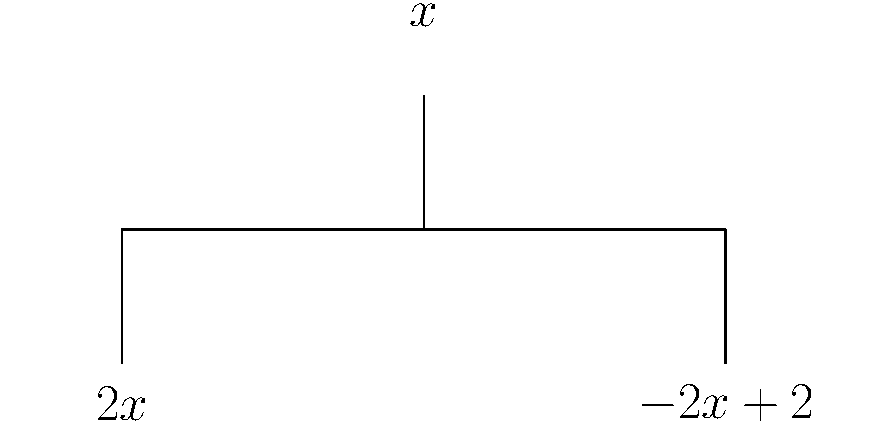
\includegraphics[scale=0.45]{../TeXGraph/Pdf/visuel_2D_arbre.pdf}
\captionof{figure}{\emph{L'arbre des positions possibles de $x$ après une étape}.}
\end{center}
On remarque que $2x$ en binaire correspond à un décalage de la virgule d'un cran vers la droite. De même, $2-2x$ est le complémentaire à $2$ de $2x$ donc, en binaire cela correspond à décaler la virgule d'un cran vers la droite puis à remplacer les $0$ par des $1$ et les $1$ par des $0$. Voici quelque exemple :
\hypertarget{9}{}
\[\begin{cases}\frac{2}{5}=\overline{0{,}0110\ldots}^{\left(2\right)}&\text{ et }f\left(\frac{2}{5}\right)=\frac{4}{5}=\overline{0{,}1100\ldots}^{\left(2\right)}\\\frac{8}{9}=\overline{0{,}111000\ldots}^{\left(2\right)}&\text{ et }f\left(\frac{8}{9}\right)=\frac{2}{9}=\overline{0{,}001110\ldots}^{\left(2\right)}\\\frac{7}{9}=\overline{0{,}110001\ldots}^{\left(2\right)}&\text{ et }f\left(\frac{7}{9}\right)=\frac{4}{9}=\overline{0{,}011100\ldots}^{\left(2\right)}\hypertarget{13}{}\\\frac{7}{12}=\overline{0{,}1001\ldots}^{\left(2\right)}&\text{ et }f\left(\frac{7}{12}\right)=\frac{10}{12}=\frac{5}{6}=\overline{0{,}110\ldots}^{\left(2\right)}\end{cases}\]

Noter toutefois que dans le dernier cas, seuls les blocs $01$ et $10$ se répètent. Nous verrons plus tard pourquoi ces deux positions en binaire ne sont pas \emph{entièrement} périodiques.

\subsubsection{La présence de cycles, une classification des rationnels en base 2}
Des \hyperlink{9}{exemples} précédents il semblerait que tout rationnel de $\left[0;1\right]$ a soit une écriture binaire finie (ce qui est le cas de $0$ et de $\frac{1}{2^n}$ avec $n\in\mathbb{N}$) soit une écriture binaire périodique\footnote{Attention à ne pas confondre position périodique en binaire (qui correspondent aux positions périodiques dans la pâte feuilletée) et position binaire périodique (qui correspondent aux positions dont les chiffres après la virgule se répètent).} soit un \emph{mélange}\footnote{Le \hyperlink{13}{dernier exemple} de la précédente partie nous laisserai supposer que les positions -- sous forme irréductible -- qui ont un dénominateur pair (autre qu'une puissance de deux) sont composées d'une partie finie de chiffres suivie d'une répétition d'un même bloc de chiffres.} des deux. On distingue trois cas (on supposera dans les trois cas que les fractions données sont irréductibles) :

\begin{enumerate}
\item\textbf{Le cas $r=\frac{p}{2^n}$} (avec des entiers $n>0$ et $p\in\left\llbracket0;2^n-1\right\rrbracket$)

On pose $p=2^mr_m+2^{m-1}r_{m-1}+\ldots+2r_1+r_0$ avec un entier positif $m$ et $r_0,r_1,r_2,\ldots,r_{m}\in\left\{0;1\right\}$. On obtient
\[r=\frac{p}{2^n}=\frac{2^mr_m+2^{m-1}r_{m-1}+\ldots+2r_1+r_0}{2^n}=\frac{r_m}{2^{n-m}}+\frac{r_{m-1}}{2^{n-m+1}}+\ldots+\frac{r_1}{2^{n-1}}+\frac{r_0}{2^n}\]
et d'après la \hyperlink{5}{\textbf{propriété 2}} : $r=\overline{0{,}\underbrace{0\ldots0}_{n-m-1\text{ fois}}r_mr_{m-1}\ldots r_1r_0}^{\left(2\right)}$. C'est l'expression en binaire de $r$ et on remarque que celle-ci est finie.
\item\textbf{Le cas $r=\frac{p}{q}$} (avec des entiers $q>1$, $q$ impair et $p\in\left\llbracket1;q-1\right\rrbracket$)

On pose le résultat :

\newprop{Soit un entier impair $q>1$ alors il existe un entier $m>0$ tel que $qm+1$ soit une puissance entière de $2$.}

\newPreuve{Puisque $\operatorname{PGCD}\left(q;2\right)=1$ alors d'après
le \href{https://fr.wikipedia.org/wiki/Th\%C3\%A9or\%C3\%A8me_d\%27Euler\_(arithm\%C3\%A9tique)}{théorème d'Euler} $2^{\varphi\left(q\right)}-1\equiv0\pmod{q}$. Il suffit alors de prendre $m=\frac{2^{\varphi\left(q\right)}-1}{q}$ et ainsi $qm+1$ est une puissance entière de $2$.}

\newcoro{Tout rationnel $0<r<1$ dont le dénominateur (sous forme irréductible) est impair à une écriture binaire périodique}

\newPreuve{On pose $r=\frac{p}{q}$ où $p$ et $q$ satisfont les hypothèses de l'énoncer. D'après \hyperlink{14}{\emph{le résultat}} de la partie suivante en multipliant le numérateur et le dénominateur par $\frac{2^{\varphi\left(q\right)}-1}{q}$, on obtient $r=\frac{p}{q}=\frac{p\times\frac{\left(2^{\varphi\left(q\right)}-1\right)}{q}}{2^{\varphi\left(q\right)}-1}$. On converti alors le numérateur en binaire, disons $p\times\frac{\left(2^{\varphi\left(q\right)}-1\right)}{q}=\overline{r_0r_1\ldots r_{m-1}r_m}^{\left(2\right)}$ avec $m\in\mathbb{N}$ et $r_0,r_1,\ldots,r_m\in\left\{0;1\right\}$ alors $r=\overline{0{,}r_0r_1\ldots r_mr_0\ldots r_m\ldots}^{\left(2\right)}$ et le bloc $r_0\ldots r_m$ est périodique.}

\item\textbf{Le cas $r=\frac{p}{2^nq}$} (avec des entiers $q>1$, $q$ impair, $n\in\mathbb{N}^*$ et $p\in\left\llbracket1;2^nq-1\right\rrbracket$)

D'après la \hyperlink{15}{\textbf{propriété 1}} on pose $p=bq+r^{\prime}$ avec $0\leqslant r^{\prime}<q$ et $b\in\mathbb{N}$ ainsi $r=\frac{p}{2^nq}=\frac{b}{2^n}+\frac{r^{\prime}}{2^nq}$. Des cas \textbf{1)} et \textbf{2)} précédents on en déduit l'existence d'entiers $r_0,r_1,\ldots,r_{n-1},r^{\prime}_0,r^{\prime}_1,\ldots,r^{\prime}_m\in\left\{0;1\right\}$ avec $m\in\mathbb{N}$ tel que $\frac{b}{2^n}=\overline{0{,}r_0r_1\ldots r_{n-1}}^{\left(2\right)}$ et $\frac{r^{\prime}}{2^nq}=\overline{0{,}\underbrace{0\ldots0}_{n\text{ fois}}r^{\prime}_0r^{\prime}_1\ldots r^{\prime}_mr^{\prime}_1\ldots r^{\prime}_m\ldots}^{\left(2\right)}$ ainsi\footnote{En binaire, diviser un réel par $2$ revient à décaler la virgule d'un cran vers la gauche.} $r=\overline{0{,}r_0r_1\ldots r_{n-1}r^{\prime}_0r^{\prime}_1\ldots r^{\prime}_mr^{\prime}_1\ldots r^{\prime}_m\ldots}^{\left(2\right)}$ et c'est bien un composé des deux cas précédents.
\end{enumerate}

Cette étude nous montre que toutes positions rationnelles en binaire est soient finie (uniquement si le dénominateur est une puissance entière de $2$ ou si la position est nulle) soit périodique (uniquement si le dénominateur est un entier positif impair) soit composée d'une partie finie suivi d'une partie périodique.

\subsection{L'étude des positions binaires périodiques}
Dans cette partie, nous allons voir en quoi l'approche binaire nous permet d'étudier plus facilement les positions périodiques. Tout d'abord, nous verrons comment passer de la base $2$ à la base $10$ puis nous trouverons une nouvelle façon d'exprimer les positions périodiques.
\subsubsection{Le passage de base $2$ à base $10$}
Le passage de la base $2$ à la base $10$ s'effectue grâce à la \hyperlink{5}{\textbf{propriété 2}}. En effet, soit $0<r<1$ un réel tel que $r=\overline{0{,}r_1r_2r_3\ldots}^{\left(2\right)}$ avec $r_1,r_2,r_3,\ldots\in\left\{0;1\right\}$ alors en base $10$ $r=\frac{r_1}{2}+\frac{r_2}{2^2}+\frac{r_3}{2^3}+\ldots$ 

Nous avons aussi fait un programme qui, à partir d'une position binaire finie ou périodique, renvoi son écriture en base $10$. Pour le comprendre, cherchons à écrire en base $10$ une position binaire finie c'est-à-dire de la forme $r=\overline{r_1r_2r_3\ldots r_n}^{\left(2\right)}$ avec $r_1,r_2,r_3,\ldots\in\left\{0;1\right\}$ et un entier $n>0$. D'après la \hyperlink{5}{propriété $2$}, 
\[r=\frac{r_1}{2}+\frac{r_2}{2^2}+\ldots+\frac{r_n}{2^n}=\frac{2^{n-1}r_1+2^{n-2}r_2+\ldots+2r_{n-1}+r_n}{2^n}\]
(on met toutes les fractions sous un même dénominateur : $2^n$). Il suffit alors de calculer le numérateur et le dénominateur pour connaître $r$ en base $10$. 
\hypertarget{14}{}
Pour les positions binaires périodiques on procède de la manière suivante. Soit $r_1,r_2,r_3,\ldots r_n$ des entiers (avec $n>0$ un entier) de l'ensemble $\left\{0;1\right\}$ on s'intéresse à l'écriture en base $10$ du réel :
\[r=\overline{0,r_1r_2r_3\ldots r_nr_1r_2\ldots r_n\ldots}^{\left(2\right)}\]
où le bloc $r_1r_2r_3\ldots r_n$ se répète indéfiniment. Donc, d'après la \hyperlink{5}{\textbf{propriété 2}} :
\[r=\frac{r_1}{2}+\frac{r_2}{2^2}+\frac{r_3}{2^3}+\ldots+\frac{r_n}{2^n}+\frac{r_1}{2^{n+1}}+\frac{r_2}{2^{n+2}}+\ldots+\frac{r_n}{2^{2n}}+\ldots\]
et en multipliant $r$ par $2^n$ on obtient 
\begin{align*}
2^nr&=2^{n-1}r_1+2^{n-2}r_2+\ldots+2r_{n-1}+r_n+\frac{r_1}{2}+\frac{r_2}{2^2}+\frac{r_3}{2^3}+\ldots+\frac{r_n}{2^n}+\frac{r_1}{2^{n+1}}+\ldots\\
&=2^{n-1}r_1+2^{n-2}r_2+\ldots+2r_{n-1}+r_n+r
\end{align*}
donc\footnote{Ce résultat s'obtient aussi en considérant la somme infinie ${\displaystyle\lim_{t\to+\infty}\sum_{k=0}^t\left(\frac{r_1}{2}+\frac{r_2}{2^2}+\ldots+\frac{r_n}{2^n}\right)\times\frac{1}{2^{kn}}}={\displaystyle\lim_{t\to+\infty}\left(\frac{r_1}{2}+\frac{r_2}{2^2}+\ldots+\frac{r_n}{2^n}\right)\times\sum_{k=0}^t\frac{1}{2^{kn}}}$ qui est convergente pour un entier $n>0$. C'est la somme des termes d'une suite géométrique de premier terme $1$ et de raison $\frac{1}{2^n}$.}
\hypertarget{11}{}
\[r=\frac{2^{n-1}r_1+2^{n-2}r_2+\ldots+2r_{n-1}+r_n}{2^n-1}\]
Ici aussi il suffit de calculer le numérateur et le dénominateur pour connaître $r$ en base $10$. Voici l'algorithme :

\begin{center}
\begin{minted}[frame=lines,breaklines,framesep=12pt,baselinestretch=1.2,bgcolor=bg,fontsize=\footnotesize,linenos]{text}
Définir une chaîne binaire,
Définir un booléen périodique (si le bloc de chiffres 'binaire' se répète),
Définir un booléen irréductible (si la fraction renvoyée devra être irréductible),
Définir un numérateur et le mettre à 0,
Définir un dénominateur et le mettre à 1,
Pour chaque chiffre de 'binaire' à l'envers : (pour plus de rapidité)
    Multiplier le chiffre par 'dénominateur' et l'ajouter à 'numérateur',
    Multiplier 'dénominateur' par 2,
    
Si 'périodique' est vraie :
    Si 'irréductible' est vraie :
        Renvoyer la fraction irréductible 'numérateur'/('dénominateur'-1).
    Sinon :
        Renvoyer la fraction 'numérateur'/(dénominateur'-1).
Sinon : 
    Si 'irréductible' est vraie :
        Renvoyer la fraction irréductible 'numérateur'/'dénominateur'.
    Sinon :
        Renvoyer la fraction 'numérateur'/'dénominateur'.
\end{minted}
\captionof{figure}{\emph{Algorithme pour passer de base $2$ à base $10$ (chez les rationnels)}.}
\end{center}

À la ligne $6$, nous parcourons la chaîne \emph{binaire} à l'envers. Cela vient du fait que le numérateur recherché est de la forme $2^{n-1}r_1+2^{n-2}r_2+\ldots+2r_{n-1}+r_n$ où la chaîne \emph{binaire} vaut $r_1r_2r_3\ldots r_n$. Ainsi, aux lignes $7$ et $8$, on multiplie progressivement\footnote{Cette étape est moins gourmande en temps et en mémoire car calculer chacun des $2^i$ pour $i\in\left\llbracket0;n\right\rrbracket$ demande beaucoup de temps.} le dénominateur par $2$. Puis, une fois en possession du numérateur et du dénominateur, on utilisera le module \href{https://docs.python.org/3.6/library/fractions.html}{\emph{fractions}} de Python qui permet de rendre une fraction sous forme irréductible. De cet algorithme on construit notre programme\footnote{On laissera au lecteur le loisir de voir que les programmes de conversions base $2$ base $10$ et \emph{vice versa} donnent des résultats cohérents.} (en Python) :

\begin{center}
\begin{minted}[frame=lines,breaklines,framesep=12pt,baselinestretch=1.2,bgcolor=bg,fontsize=\footnotesize,linenos]{python}
from fractions import Fraction

def binaire_vers_decimale(binaire,periodique=False,irreductible=False):
    '''Renvoie le rationnel (entre 0 et 1) en base 10 de 'binaire'. 
       Si le bloc de chiffres 'binaire' est périodique mettre 'periodique' à 'True'.
       Le rationnel renvoyé est un tuple numérateur/dénominateur.
       Si 'irreductible' vaut 'True', la fractions renvoyée est irréductible.
    '''
    num=0 # Le numérateur du rationnel.
    den=1 # Le dénominateur du rationnel.
    for chiffre in binaire[::-1]: # Pour parcourir 'binaire' à l'envers.
        num+=int(chiffre)*den # Calcul du numérateur.
        den*=2 # On multiplie le dénominateur par 2 (soucis de rapidité).
    if periodique:
        if irreductible:return Fraction(num,den-1) # Si la fraction doit être irréductible.
        return str(num)+"/"+str(den-1) # On retourne la fraction.
    if irreductible:return Fraction(num,den) # Si la fraction doit être irréductible.
    return str(num)+"/"+str(den) # On retourne la fraction.

\end{minted}
\captionof{figure}{\emph{Code source du programme Python}.}
\end{center}

\subsubsection{Une nouvelle forme pour les positions périodiques}
Nous allons maintenant nous intéresser aux positions périodiques en base $2$.

D'après la formule obtenue à \hyperlink{11}{la partie précédente}, on remarque que celle-ci est très proche de la forme des positions périodiques. En effet, si l'on considère que $r_n=0$ alors
\[r=\overline{0{,}r_1r_2\ldots r_nr_1\ldots r_n\ldots}^{\left(2\right)}=\frac{2\left(2^{n-2}r_1+2^{n-3}r_2+\ldots+r_{n-1}\right)}{2^n-1}\]
et c'est une position périodique car $2^{n-2}r_1+\ldots2r_{n-2}+r_{n-1}$ avec $r_1,r_2,\ldots r_{n-1}\in\left\{0;1\right\}$ représente tous les entiers de $0$ à $2^{n-1}$. Et pour les positions périodiques de la forme $\frac{2k}{2^n+1}$ avec $k\in\left\llbracket1;2^{n-1}\right\rrbracket$ on multiplie en haut et en bas par $2^n-1$, on obtient $\frac{2k\times\left(2^n-1\right)}{2^{2n}-1}$ donc les toutes les positions périodiques peuvent s'exprimer grâce à la formule ci-dessus.
\section{Remerciements}
Merci à Charles Dossal, chercheur à l’Institut de Mathématiques de Toulouse, pour ce sujet et pour les questions supplémentaires, ne faisant intervenir que de la réflexion.

Merci à nos professeurs grâce à qui l’atelier MATh.en.JEANS est rendu possible.
\fancyfoot[C]{\textbf{Page \thepage/\pageref{LastPage}}}

\end{document}
